% use xelatex

\documentclass[a4paper,10pt,twocolumn,oneside]{article}
\setlength{\columnsep}{10pt}                                                              %兩欄模式的間距
\setlength{\columnseprule}{0pt}                                                                %兩欄模式間格線粗細

\usepackage{amsthm}								%定義,例題
\usepackage{amssymb}
%\usepackage[margin=2cm]{geometry}
\usepackage{fontspec}								%設定字體
\usepackage{color}
\usepackage[x11names]{xcolor}
\usepackage{listings}								%顯示code用的
%\usepackage[Glenn]{fncychap}						%排版,頁面模板
\usepackage{fancyhdr}								%設定頁首頁尾
\usepackage{graphicx}								%Graphic
\usepackage{enumerate}
\usepackage{titlesec}
\usepackage{amsmath}
\usepackage{tikz}
\usepackage[CheckSingle, CJKmath]{xeCJK}
% \usepackage{CJKulem}
%\usepackage[T1]{fontenc}
\titlespacing{\section}{0cm}{0cm}{0cm}
\titlespacing{\subsection}{0cm}{0cm}{0cm}
\usepackage{amsmath, courier, listings, fancyhdr, graphicx}
\topmargin=0pt
\headsep=5pt
\textheight=780pt
\footskip=0pt
\voffset=-40pt
\textwidth=545pt
\marginparsep=0pt
\marginparwidth=0pt
\marginparpush=0pt
\oddsidemargin=0pt
\evensidemargin=0pt
\hoffset=-42pt
\setmainfont [
    Path = .fonts/ttf/,
    UprightFont = *-Regular,
    BoldFont = *-Bold,
    ItalicFont = *-Italic
  ] {Consolas}

\setmonofont [        
    Path = .fonts/ttf/,
    UprightFont = *-Regular,
  ] {Monaco}


%\renewcommand\listfigurename{圖目錄}
%\renewcommand\listtablename{表目錄} 

%%%%%%%%%%%%%%%%%%%%%%%%%%%%%

%\setCJKmainfont{微軟正黑體}
\setCJKmainfont[
    Path = .fonts/ttf/,
    UprightFont = *,
    BoldFont = *bd,
    ItalicFont = *l
]{msjh}

\XeTeXlinebreaklocale "zh"
\XeTeXlinebreakskip = 0pt plus 1pt				%設定段落之間的距離
\setcounter{secnumdepth}{3}						%目錄顯示第三層

%%%%%%%%%%%%%%%%%%%%%%%%%%%%%
\makeatletter
\lst@CCPutMacro\lst@ProcessOther {"2D}{\lst@ttfamily{-{}}{-{}}}
\@empty\z@\@empty
\makeatother
\lstset{											% Code顯示
language=C++,										% the language of the code
basicstyle=\footnotesize\ttfamily, 						% the size of the fonts that are used for the code
%numbers=left,										% where to put the line-numbers
numberstyle=\footnotesize,						% the size of the fonts that are used for the line-numbers
stepnumber=1,										% the step between two line-numbers. If it's 1, each line  will be numbered
numbersep=5pt,										% how far the line-numbers are from the code
backgroundcolor=\color{white},					% choose the background color. You must add \usepackage{color}
showspaces=false,									% show spaces adding particular underscores
showstringspaces=false,							% underline spaces within strings
showtabs=false,									% show tabs within strings adding particular underscores
frame=false,											% adds a frame around the code
tabsize=2,											% sets default tabsize to 2 spaces
captionpos=b,										% sets the caption-position to bottom
breaklines=true,									% sets automatic line breaking
breakatwhitespace=false,							% sets if automatic breaks should only happen at whitespace
escapeinside={\%*}{*)},							% if you want to add a comment within your code
morekeywords={*},									% if you want to add more keywords to the set
keywordstyle=\bfseries\color{Blue1},
commentstyle=\itshape\color{Red4},
stringstyle=\itshape\color{Green4},
}

%%%%%%%%%%%%%%%%%%%%%%%%%%%%%

\begin{document}
\pagestyle{fancy}
\fancyfoot{}
%\fancyfoot[R]{\includegraphics[width=20pt]{ironwood.jpg}}
\fancyhead[L]{NTOU Suzukaze\_daisuki}
\fancyhead[R]{\thepage}
\renewcommand{\headrulewidth}{0.4pt}
\renewcommand{\contentsname}{Contents} 

\scriptsize
\tableofcontents
%%%%%%%%%%%%%%%%%%%%%%%%%%%%%
\section{Basic}
\subsection{Default code}
\lstinputlisting{basic/default_code.cpp}
\subsection{Linux 對拍}
\lstinputlisting{basic/stress_test_Linux.sh}
\subsection{Windows 對拍}
\lstinputlisting{basic/stress_test_Windows.bat}
\subsection{builtin 函數}
\lstinputlisting{basic/builtin_function.cpp}
\subsection{輸入輸出}
\lstinputlisting{basic/io.cpp}
\subsection{Python 輸入輸出}
\lstinputlisting{basic/py_trivial.py}

%%%%%%%%%%%%%%%%%%%%%%%%%%%%%
\section{Data Structure}
%\subsection{Link-Cut Tree}
%\lstinputlisting{datastructure/link_cut_tree.cpp}
\subsection{持久化線段樹}
\lstinputlisting{datastructure/persistent_seg_tree.cpp}
\subsection{Treap}
\lstinputlisting{datastructure/treap.cpp}
\subsection{線段樹}
\lstinputlisting{datastructure/seg_tree.cpp}
%%%%%%%%%%%%%%%%%%%%%%%%%%%%%
\section{Flow}
\subsection{Dinic}
\lstinputlisting{flow/dinic.cpp}
\subsection{匈牙利}
\lstinputlisting{flow/hungarian.cpp}
\subsection{KM}
\lstinputlisting{flow/km.cpp}
\subsection{MCMF}
\lstinputlisting{flow/mcmf.cpp}
%%%%%%%%%%%%%%%%%%%%%%%%%%%%%
\section{幾何}
\subsection{點宣告}
\lstinputlisting{geometry/pt_declare.cpp}
\subsection{矩形面積}
\lstinputlisting{geometry/area_of_rect.cpp}
\subsection{最近點對}
\lstinputlisting{geometry/closest_pair_of_points.cpp}
\subsection{凸包}
\lstinputlisting{geometry/convex_hull.cpp}
\subsection{兩直線交點}
\lstinputlisting{geometry/intersection_of_two_lines.cpp}
\subsection{兩線段交點}
\lstinputlisting{geometry/intersection_of_two_segments.cpp}
\subsection{李超線段樹}
\lstinputlisting{geometry/li_chao_seg_tree.cpp}
\subsection{最小包覆圓}
\lstinputlisting{geometry/minimal_circle.cpp}
\subsection{最小包覆球}
\lstinputlisting{geometry/minimal_ball.cpp}
\subsection{旋轉卡尺}
\lstinputlisting{geometry/rotating_caliper.cpp}
\subsection{Circle Cover }
\lstinputlisting{geometry/CircleCover.cpp}
\subsection{Convex Hull Trick}
\lstinputlisting{geometry/ConvexHulltrick.cpp}
\subsection{Half Plane Intersection}
\lstinputlisting{geometry/Half_plane_intersection.cpp}
\subsection{Minkowski Sum}
\lstinputlisting{geometry/Minkowski_Sum.cpp}
\subsection{多邊形聯集面積}
\lstinputlisting{geometry/polyUnion.cpp}
\subsection{Polygon Cover}
\lstinputlisting{geometry/PolyonCover.cpp}
\subsection{Tangent\_line\_of\_two\_circle}
\lstinputlisting{geometry/Tangent\_line\_of\_two\_circle.cpp}
\subsection{basic.cpp Revival}
\lstinputlisting{geometry/basic.cpp}
\subsection{intersection\_of\_two\_circle}
\lstinputlisting{geometry/intersection\_of\_two\_circle.cpp}


%%%%%%%%%%%%%%%%%%%%%%%%%%
\section{圖論}
\subsection{BCC}
\lstinputlisting{graph/bcc.cpp}
\subsection{重心剖分}
\lstinputlisting{graph/centroid_decom.cpp}
%\subsection{輕重鍊剖分}
%\lstinputlisting{graph/Heavy_light_decomposition.cpp}
%\subsection{歐拉路徑}
%\lstinputlisting{graph/euler_path.cpp}
\subsection{極大團}
\lstinputlisting{graph/maximal_clique.cpp}
\subsection{最大團}
\lstinputlisting{graph/maximum_clique.cpp}
\subsection{SCC}
\lstinputlisting{graph/scc.cpp}
\subsection{SPFA}
\lstinputlisting{graph/spfa.cpp}
\subsection{domainTree} 
\lstinputlisting{graph/domainTree.cpp}
\subsection{曼哈頓最小生成樹}
\lstinputlisting{graph/ManhattanMST.cpp}

\subsection{2-SAT}
($x or y$) adddege ($(x \rightarrow \neg y)$), ($(y \rightarrow \neg x)$)
\subsection{差分約束}
約束條件 : 
\begin{itemize}
    \item $V_j-V_i\le W$ addEdge($i, j, W $)
    \item $V_j-V_i\ge W$ addEdge($j, i, -W $)
    \item $V_j = V_i$ addEdge($i, j, 0 $),($j, i, 0 $)
\end{itemize}

接著跑SPFA,Bellman-Ford
%%%%%%%%%%%%%%%%%%%%%%%%%%%%%%
\section{數論}
\subsection{離散根號}
\lstinputlisting{math/discrete_sqrt.cpp}
\subsection{ex-crt}
\lstinputlisting{math/excrt.cpp}
\subsection{ex-gcd}
\lstinputlisting{math/exgcd.cpp}
\subsection{FFT}
\lstinputlisting{math/fft.cpp}
\subsection{高斯消去法}
\lstinputlisting{math/gaussian_elim.cpp}
\subsection{喬瑟夫問題}
\lstinputlisting{math/josephus.cpp}
\subsection{定理}
\begin{itemize}
    \item Lucas's Theorem :\\
      For $n, m \in \mathbb{Z}^{*}$ and prime $P$,
      $C(m,n) \mod P$
      %= C(\frac{m}{M},n/M) * C(m\%M,n\%M) mod P
        $= \Pi ( C(m_i,n_i) )$
      where $m_i$ is the $i$-th digit of $m$ in base $P$.
    \item Stirling approximation : \\
      $n!\approx\sqrt{ 2 \pi n}(\frac{n}{e})^{n}e^\frac{1}{12n}$
    \item Stirling Numbers(permutation $|P|=n$ with $k$ cycles): \\
      $S(n,k) = \text{coefficient of }x^k \text{ in } \Pi_{i=0}^{n-1} (x+i)$
    \item Stirling Numbers(Partition $n$ elements into $k$ non-empty set): \\
      $S(n,k) = \frac{1}{k!} \sum\limits_{j=0}^k (-1)^{k-j} {k \choose j} j^n$
    \item Pick's Theorem : $A = i + b/2 - 1$\\
      $A$: Area、 $i$: grid number in the inner、 $b$: grid number on the side
    \item Catalan number : $C_n = {2n \choose n}/(n+1)$\\
      $C^{n+m}_{n}-C^{n+m}_{n+1} = (m+n)! \frac{n-m+1}{n+1}\quad for \quad  n \ge m$\\
      $C_n = \frac{1}{n+1}{2n \choose n} = \frac{(2n)!}{(n+1)!n!}$\\
      $C_0 = 1 \quad  and \quad C_{n+1}= 2(\frac{2n+1}{n+2})C_n$\\
      $C_0 = 1 \quad  and \quad C_{n+1} = \sum_{i=0}^{n} C_iC_{n-i} \quad for \quad  n \ge 0$
    \item Euler Characteristic: \\
      planar graph: $V-E+F-C=1$ \\
      convex polyhedron: $V-E+F=2$ \\
      $V,E,F,C$: number of vertices, edges, faces(regions), and components
    \item Kirchhoff's theorem : \\
      $A_{ii} = deg(i), A_{ij} = (i,j) \in E\ ? -1 : 0$,
      Deleting any one row, one column, and cal the det(A)
    \item Polya' theorem ($c$ is number of color,$m$ is the number of cycle size): \\
      $(\sum_{i=1}^{m}{c^{gcd(i,m)}})/m$
    \item Burnside lemma: \\
      $|X/G| = \frac{1}{|G|}\sum\limits_{g\in G} |X^g|$
    \item 錯排公式 :  ($n$個人中,每個人皆不再原來位置的組合數): \\
      $dp[0]=1;dp[1]=0;$\\
      $dp[i]=(i-1)*(dp[i-1]+dp[i-2])$;
    \item Bell數 (有$n$個人,把他們拆組的方法總數) : \\
      $B_0= 1$\\
      $B_n= \sum_{k=0}^{n} s(n,k)\quad (second-stirling)\\
      B_{n+1}= \sum_{k=0}^{n}{n \choose k} B_k$
    \item Wilson's theorem :\\
      $(p-1)! \equiv -1 (mod \ p)$
    \item Fermat's little theorem :\\
      $a^p \equiv a (mod \ p)$
    \item Euler's totient function:\\
      $ A ^ {B ^ C} mod \ p = pow(A,pow(B,C,p-1)) mod \ p$
    \item 歐拉函數降冪公式:\\
      $A^B \mod C=A^{B \mod \phi(c) + \phi(c)}\mod C$
    \item 6的倍數: \\
     $(a-1)^3 + (a+1)^3 + (-a)^3 + (-a)^3 = 6a$
\end{itemize}
\subsection{Miller Rabin}
\lstinputlisting{math/miller_rabin.cpp}
\subsection{NTT}
\lstinputlisting{math/ntt.cpp}
\subsection{Pollard's Rho}
\lstinputlisting{math/pollard_rho.cpp}
\subsection{質數}
\lstinputlisting{math/primes.cpp}
\subsection{phi}
\lstinputlisting{math/phi.cpp}
\subsection{矩陣快速冪}
\lstinputlisting{math/matrix_fast_pow.cpp}
\subsection{矩陣相乘}
\lstinputlisting{math/matrix_multiply.cpp}

%%%%%%%%%%%%%%%%%%%%%%%%%%%%%%%
\section{字串}
\subsection{KMP}
\lstinputlisting{string/kmp.cpp}
\subsection{馬拉車}
\lstinputlisting{string/manacher.cpp}
\subsection{回文樹}
\lstinputlisting{string/pal_tree.cpp}
\subsection{SA}
\lstinputlisting{string/sa.cpp}
\subsection{SAM}
\lstinputlisting{string/sam.cpp}
\subsection{樹哈希}
\lstinputlisting{string/tree_hash.cpp}
\subsection{trie}
\lstinputlisting{string/trie.cpp}
\subsection{Z-value}
\lstinputlisting{string/z_value.cpp}
\subsection{minRotation}
\lstinputlisting{string/minrotation.cpp}
%%%%%%%%%%%%%%%%%%%%%%%%%%%%%%%
\section{DP}
\subsection{數位 dp}
\lstinputlisting{dp/digit.cpp}
\subsection{SOS dp}
\lstinputlisting{dp/sos.cpp}
\subsection{p-median}
\lstinputlisting{dp/p_median.cpp}
%%%%%%%%%%%%%%%%%%%%%%%%%%%%%%%
\section{Other}
\subsection{黑魔法、名次樹}
\lstinputlisting{other/black_magic.cpp}
%\subsection{Dancing Links}
%\lstinputlisting{other/dlx.cpp}
\subsection{Hilbert curve}
\lstinputlisting{other/hibert_curve.cpp}
%\subsection{模擬退火}
%\lstinputlisting{other/simulated_annealing.cpp}   
%%%%%%%%%%%%%%%%%%%%%%%%%%%%%%%
\makeatletter
\def\grd@save@target#1{%
  \def\grd@target{#1}}
\def\grd@save@start#1{%
  \def\grd@start{#1}}
\tikzset{
  grid with coordinates/.style={
    to path={%
      \pgfextra{%
        \edef\grd@@target{(\tikztotarget)}%
        \tikz@scan@one@point\grd@save@target\grd@@target\relax
        \edef\grd@@start{(\tikztostart)}%
        \tikz@scan@one@point\grd@save@start\grd@@start\relax
        \draw[minor help lines] (\tikztostart) grid (\tikztotarget);
        \draw[major help lines] (\tikztostart) grid (\tikztotarget);
        \grd@start
        \pgfmathsetmacro{\grd@xa}{\the\pgf@x/1cm}
        \pgfmathsetmacro{\grd@ya}{\the\pgf@y/1cm}
        \grd@target
        \pgfmathsetmacro{\grd@xb}{\the\pgf@x/1cm}
        \pgfmathsetmacro{\grd@yb}{\the\pgf@y/1cm}
        \pgfmathsetmacro{\grd@xc}{\grd@xa + \pgfkeysvalueof{/tikz/grid with coordinates/major step}}
        \pgfmathsetmacro{\grd@yc}{\grd@ya + \pgfkeysvalueof{/tikz/grid with coordinates/major step}}
        \foreach \x in {\grd@xa,\grd@xc,...,\grd@xb}
        \node[anchor=north] at (\x,\grd@ya) {\pgfmathprintnumber{\x}};
        \foreach \y in {\grd@ya,\grd@yc,...,\grd@yb}
        \node[anchor=east] at (\grd@xa,\y) {\pgfmathprintnumber{\y}};
      }
    }
  },
  minor help lines/.style={
    help lines,
    step=\pgfkeysvalueof{/tikz/grid with coordinates/minor step}
  },
  major help lines/.style={
    help lines,
    line width=\pgfkeysvalueof{/tikz/grid with coordinates/major line width},
    step=\pgfkeysvalueof{/tikz/grid with coordinates/major step}
  },
  grid with coordinates/.cd,
  minor step/.initial=.2,
  major step/.initial=1,
  major line width/.initial=2pt,
}
\makeatother

\vphantom
\newline
\newpage
\vphantom
\newline
\newpage
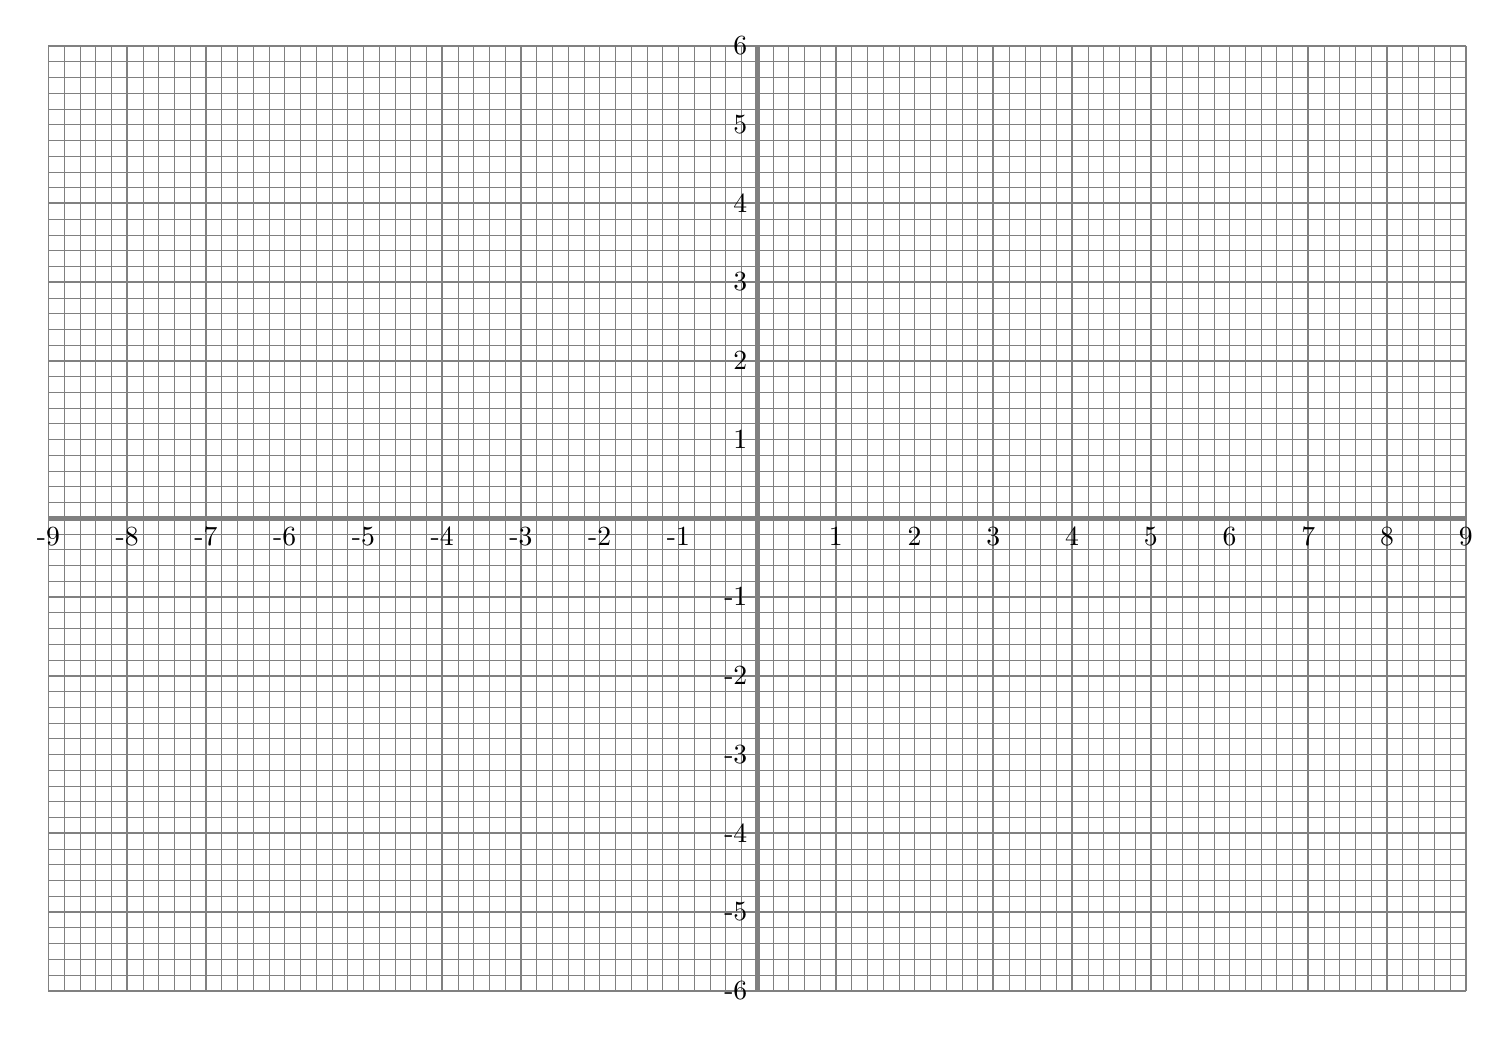
\begin{tikzpicture}
\draw[help lines,step=.2] (-9,-6) grid (9,6);
\draw[help lines,line width=.6pt,step=1] (-9,-6) grid (9,6);
\draw[help lines,line width=1.8pt,step=1] (0,-6) grid (0,6);
\draw[help lines,line width=1.8pt,step=1] (-9,0) grid (9,0);
\foreach \x in {-9,-8,-7,-6,-5,-4,-3,-2,-1, ,1,2,3,4,5,6,7,8,9}
 \node[anchor=north] at (\x,0) {\x};
\foreach \y in {-6,-5,-4,-3,-2,-1, ,1,2,3,4,5,6}
 \node[anchor=east] at (0,\y) {\y};
\end{tikzpicture}

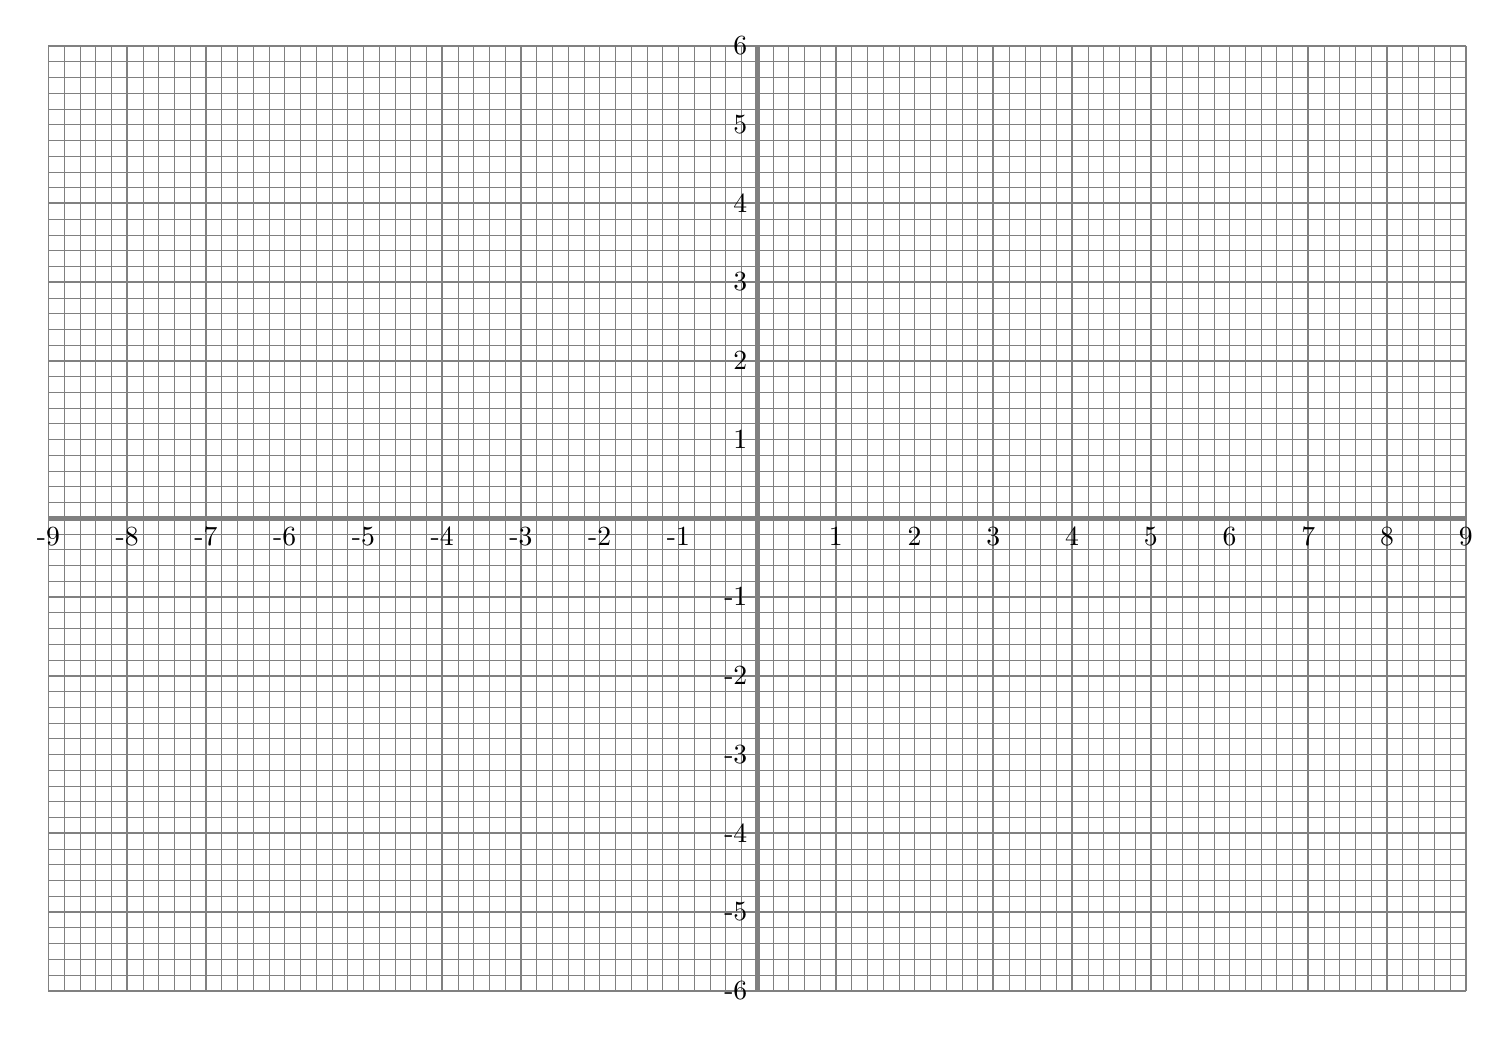
\begin{tikzpicture}
\draw[help lines,step=.2] (-9,-6) grid (9,6);
\draw[help lines,line width=.6pt,step=1] (-9,-6) grid (9,6);
\draw[help lines,line width=1.8pt,step=1] (0,-6) grid (0,6);
\draw[help lines,line width=1.8pt,step=1] (-9,0) grid (9,0);
\foreach \x in {-9,-8,-7,-6,-5,-4,-3,-2,-1, ,1,2,3,4,5,6,7,8,9}
 \node[anchor=north] at (\x,0) {\x};
\foreach \y in {-6,-5,-4,-3,-2,-1, ,1,2,3,4,5,6}
 \node[anchor=east] at (0,\y) {\y};
\end{tikzpicture}

\vphantom
\newline
\newpage
\vphantom
\newline
\newpage
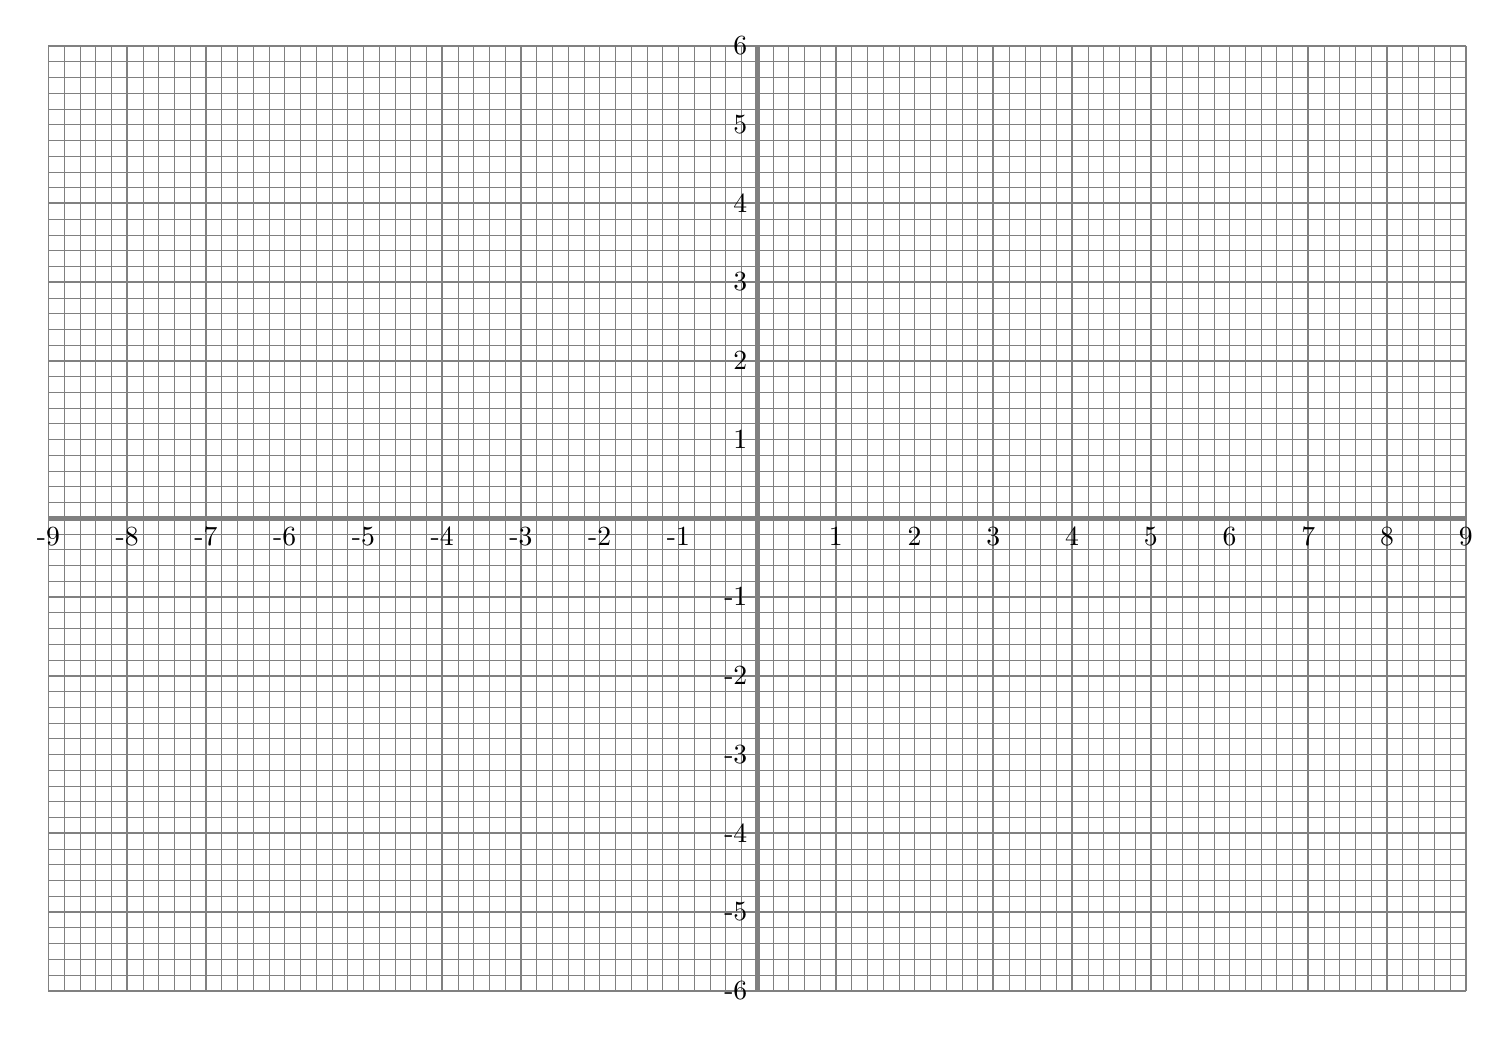
\begin{tikzpicture}
\draw[help lines,step=.2] (-9,-6) grid (9,6);
\draw[help lines,line width=.6pt,step=1] (-9,-6) grid (9,6);
\draw[help lines,line width=1.8pt,step=1] (0,-6) grid (0,6);
\draw[help lines,line width=1.8pt,step=1] (-9,0) grid (9,0);
\foreach \x in {-9,-8,-7,-6,-5,-4,-3,-2,-1, ,1,2,3,4,5,6,7,8,9}
 \node[anchor=north] at (\x,0) {\x};
\foreach \y in {-6,-5,-4,-3,-2,-1, ,1,2,3,4,5,6}
 \node[anchor=east] at (0,\y) {\y};
\end{tikzpicture}

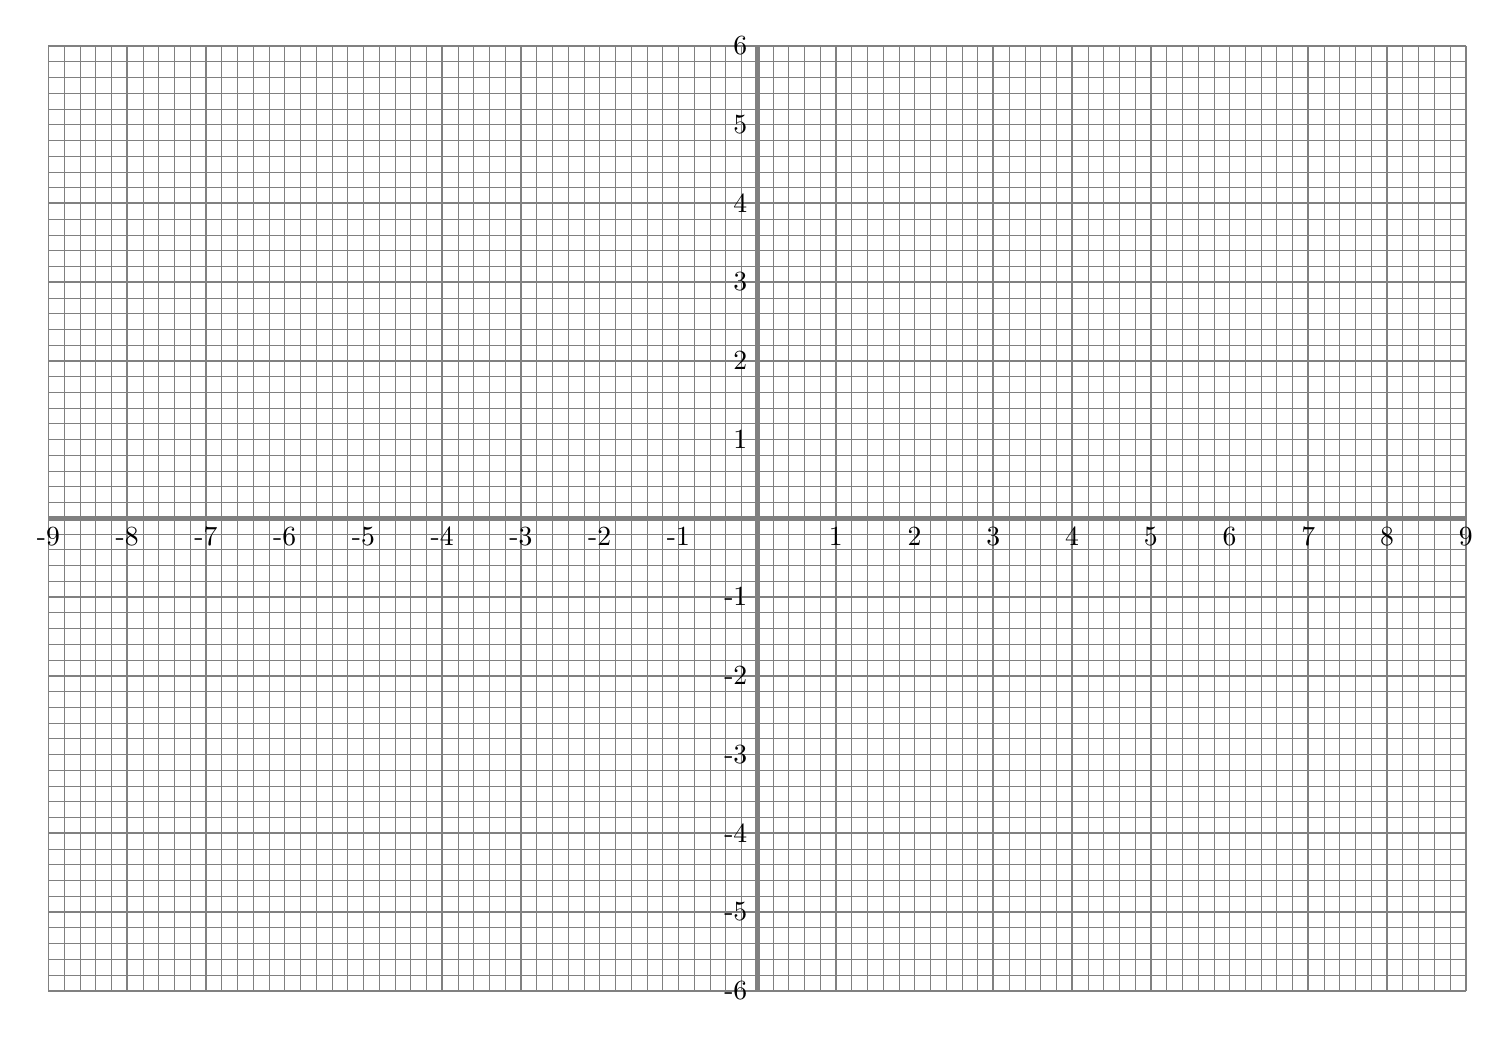
\begin{tikzpicture}
\draw[help lines,step=.2] (-9,-6) grid (9,6);
\draw[help lines,line width=.6pt,step=1] (-9,-6) grid (9,6);
\draw[help lines,line width=1.8pt,step=1] (0,-6) grid (0,6);
\draw[help lines,line width=1.8pt,step=1] (-9,0) grid (9,0);
\foreach \x in {-9,-8,-7,-6,-5,-4,-3,-2,-1, ,1,2,3,4,5,6,7,8,9}
 \node[anchor=north] at (\x,0) {\x};
\foreach \y in {-6,-5,-4,-3,-2,-1, ,1,2,3,4,5,6}
 \node[anchor=east] at (0,\y) {\y};
\end{tikzpicture}
\vphantom
\newline
\newpage
\vphantom
\newline
\newpage
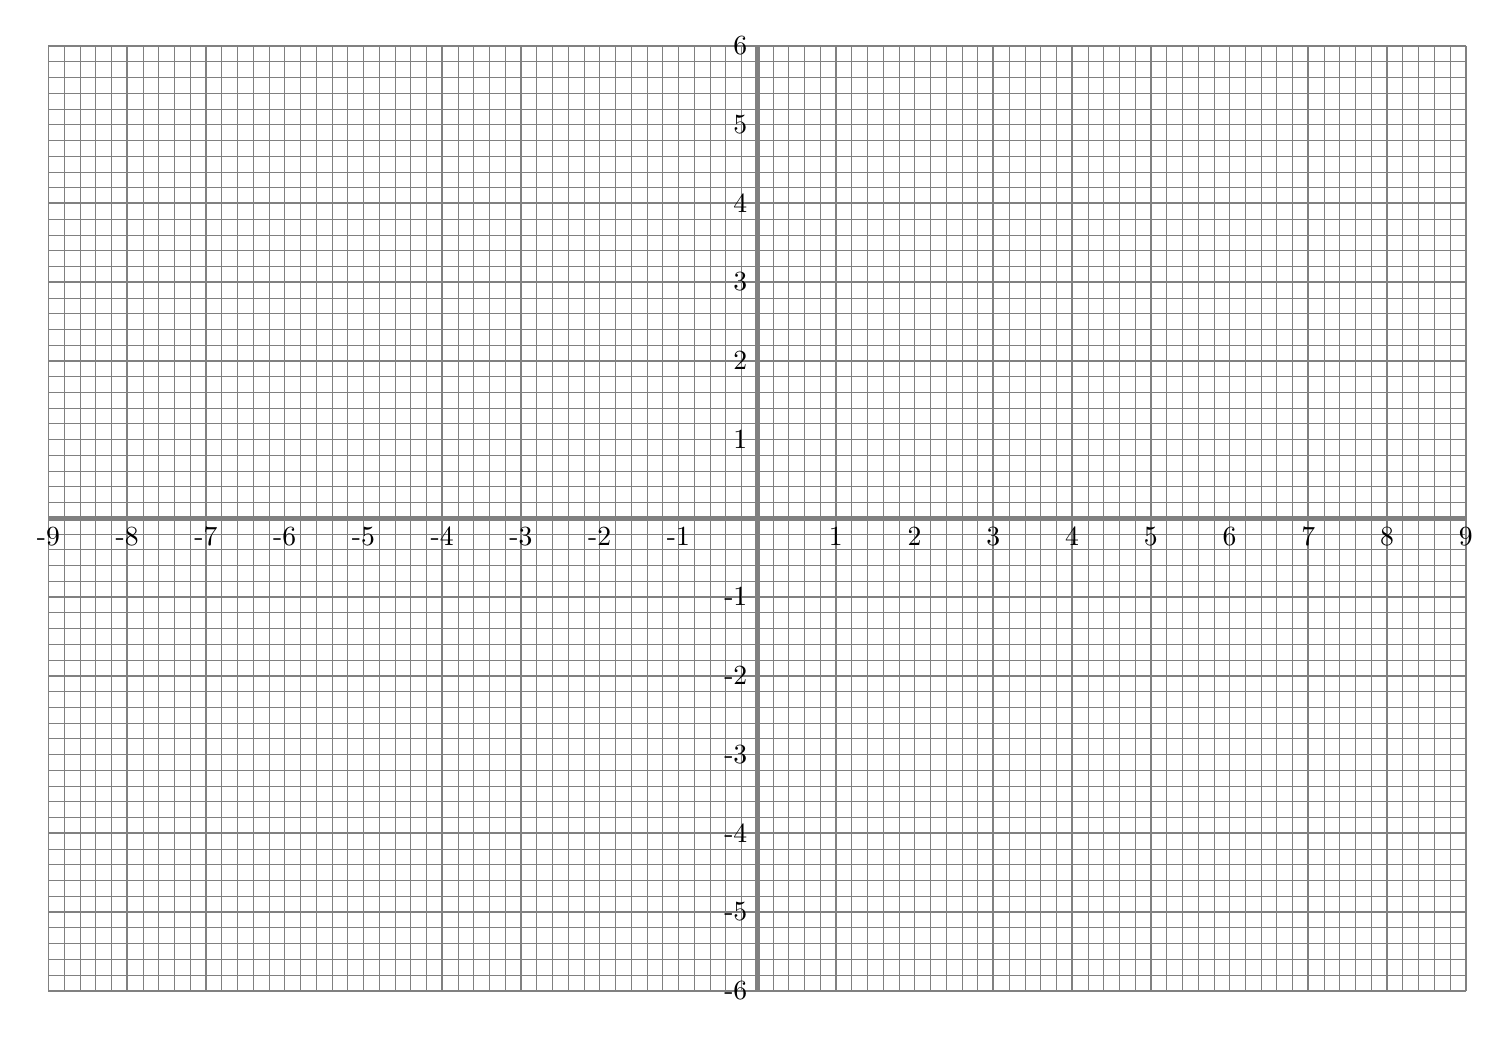
\begin{tikzpicture}
\draw[help lines,step=.2] (-9,-6) grid (9,6);
\draw[help lines,line width=.6pt,step=1] (-9,-6) grid (9,6);
\draw[help lines,line width=1.8pt,step=1] (0,-6) grid (0,6);
\draw[help lines,line width=1.8pt,step=1] (-9,0) grid (9,0);
\foreach \x in {-9,-8,-7,-6,-5,-4,-3,-2,-1, ,1,2,3,4,5,6,7,8,9}
 \node[anchor=north] at (\x,0) {\x};
\foreach \y in {-6,-5,-4,-3,-2,-1, ,1,2,3,4,5,6}
 \node[anchor=east] at (0,\y) {\y};
\end{tikzpicture}

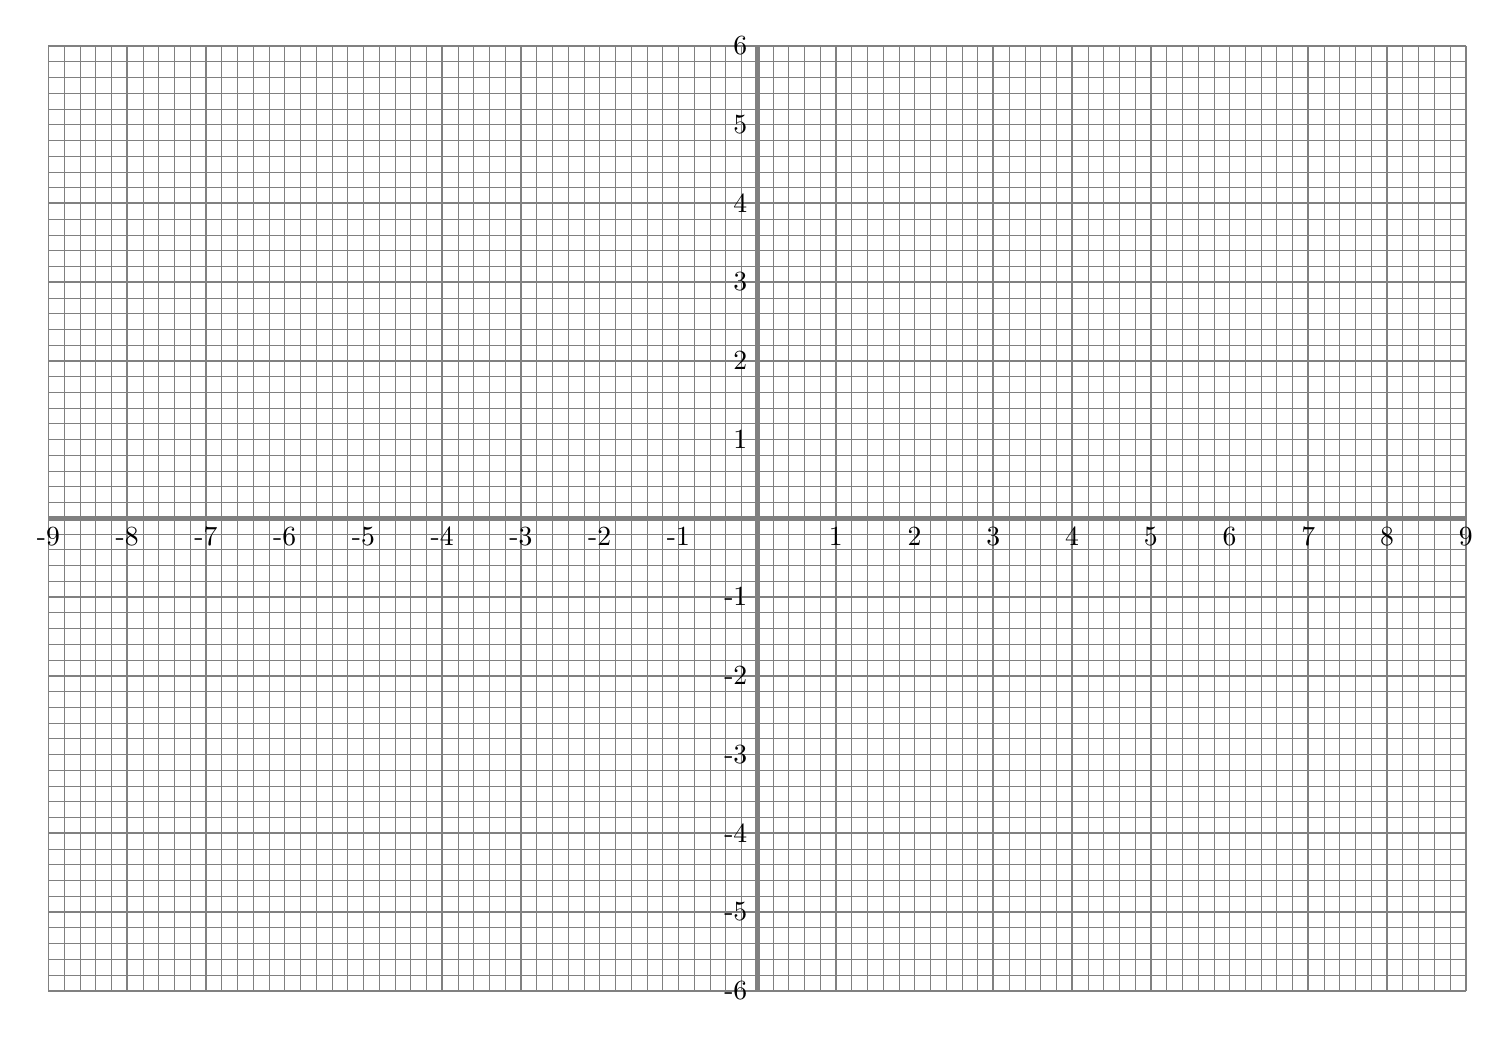
\begin{tikzpicture}
\draw[help lines,step=.2] (-9,-6) grid (9,6);
\draw[help lines,line width=.6pt,step=1] (-9,-6) grid (9,6);
\draw[help lines,line width=1.8pt,step=1] (0,-6) grid (0,6);
\draw[help lines,line width=1.8pt,step=1] (-9,0) grid (9,0);
\foreach \x in {-9,-8,-7,-6,-5,-4,-3,-2,-1, ,1,2,3,4,5,6,7,8,9}
 \node[anchor=north] at (\x,0) {\x};
\foreach \y in {-6,-5,-4,-3,-2,-1, ,1,2,3,4,5,6}
 \node[anchor=east] at (0,\y) {\y};
\end{tikzpicture}

\vphantom
\newline
\newpage
\vphantom
\newline
\newpage
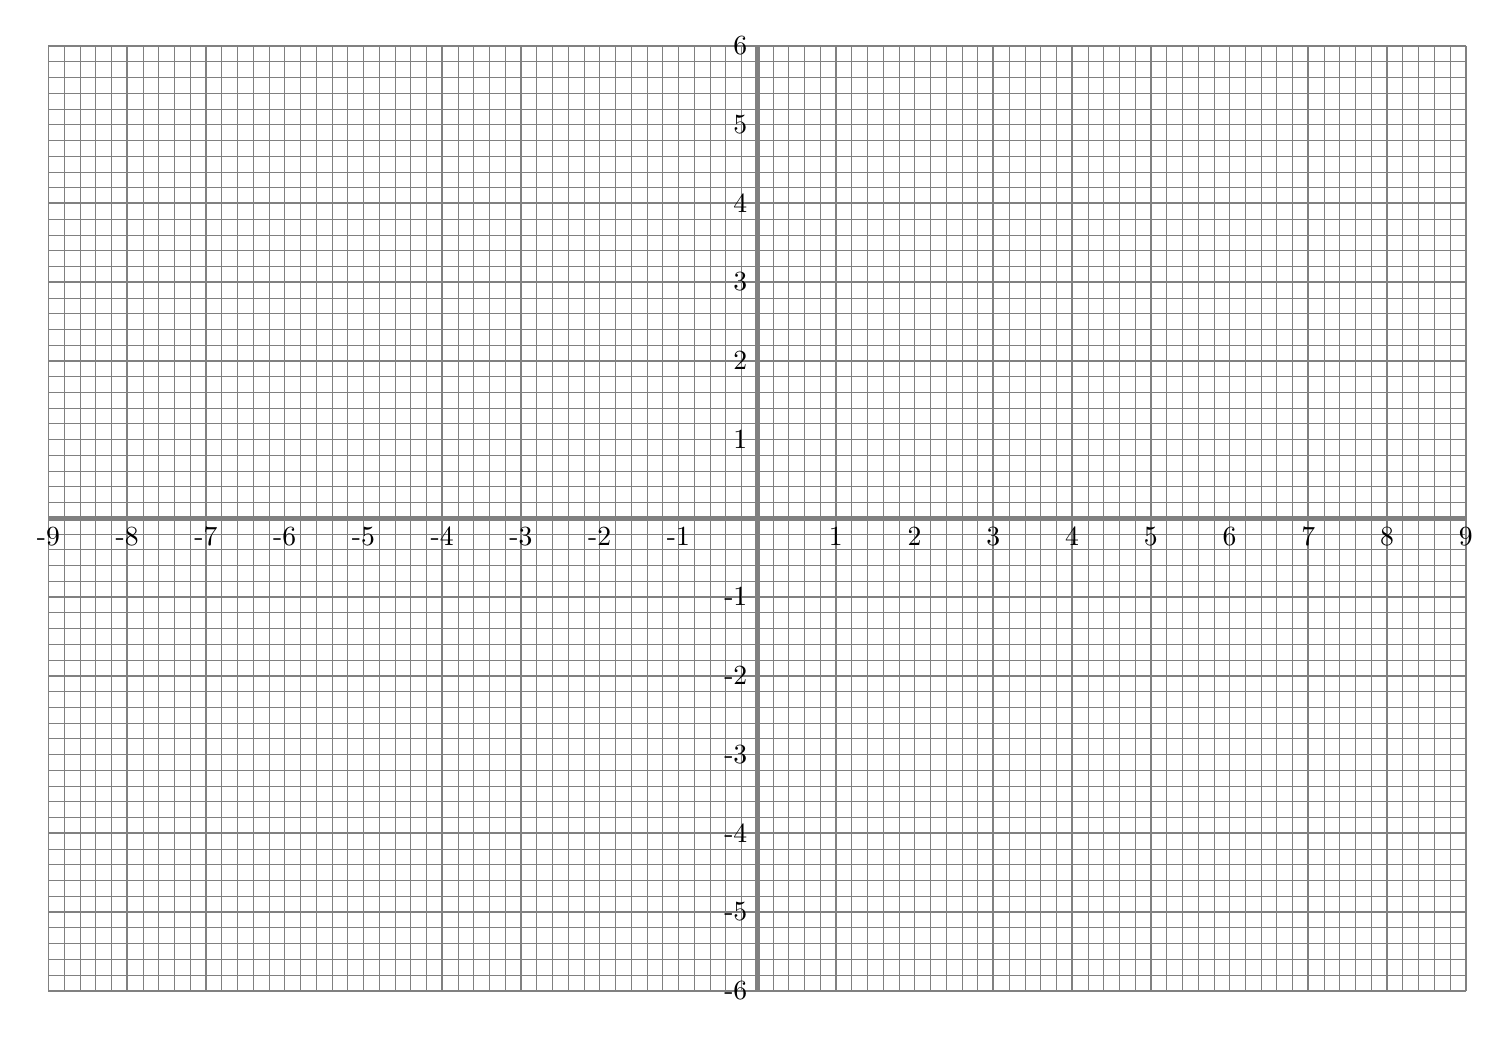
\begin{tikzpicture}
\draw[help lines,step=.2] (-9,-6) grid (9,6);
\draw[help lines,line width=.6pt,step=1] (-9,-6) grid (9,6);
\draw[help lines,line width=1.8pt,step=1] (0,-6) grid (0,6);
\draw[help lines,line width=1.8pt,step=1] (-9,0) grid (9,0);
\foreach \x in {-9,-8,-7,-6,-5,-4,-3,-2,-1, ,1,2,3,4,5,6,7,8,9}
 \node[anchor=north] at (\x,0) {\x};
\foreach \y in {-6,-5,-4,-3,-2,-1, ,1,2,3,4,5,6}
 \node[anchor=east] at (0,\y) {\y};
\end{tikzpicture}

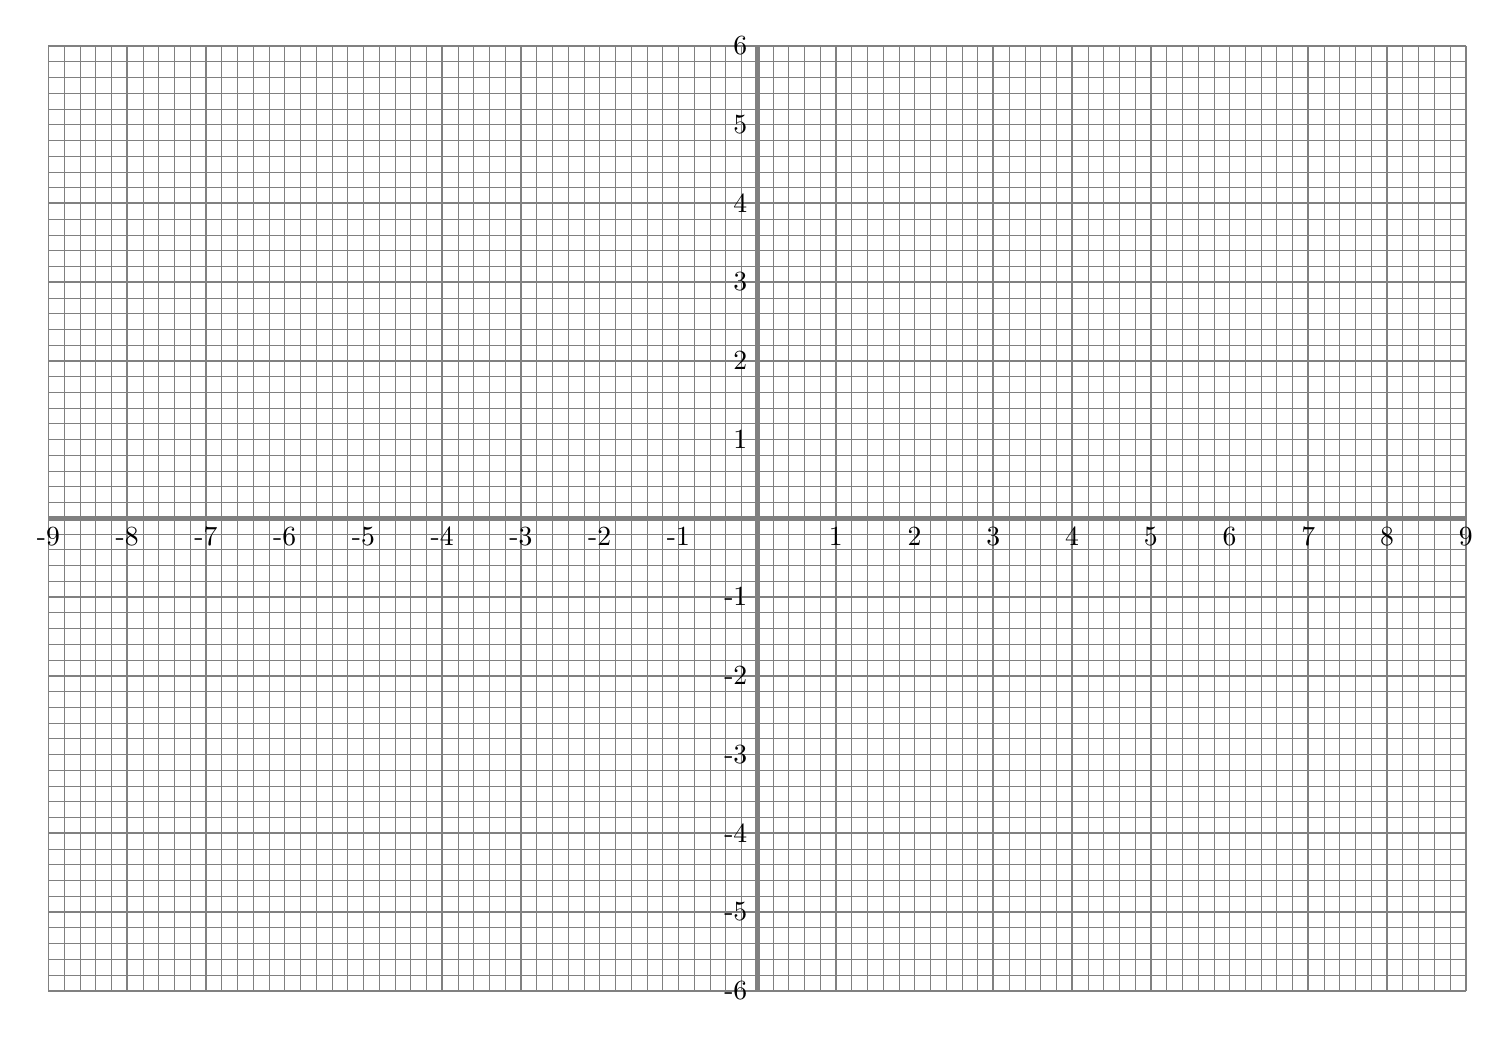
\begin{tikzpicture}
\draw[help lines,step=.2] (-9,-6) grid (9,6);
\draw[help lines,line width=.6pt,step=1] (-9,-6) grid (9,6);
\draw[help lines,line width=1.8pt,step=1] (0,-6) grid (0,6);
\draw[help lines,line width=1.8pt,step=1] (-9,0) grid (9,0);
\foreach \x in {-9,-8,-7,-6,-5,-4,-3,-2,-1, ,1,2,3,4,5,6,7,8,9}
 \node[anchor=north] at (\x,0) {\x};
\foreach \y in {-6,-5,-4,-3,-2,-1, ,1,2,3,4,5,6}
 \node[anchor=east] at (0,\y) {\y};
\end{tikzpicture}

\vphantom
\newline
\newpage
\vphantom
\newline
\newpage
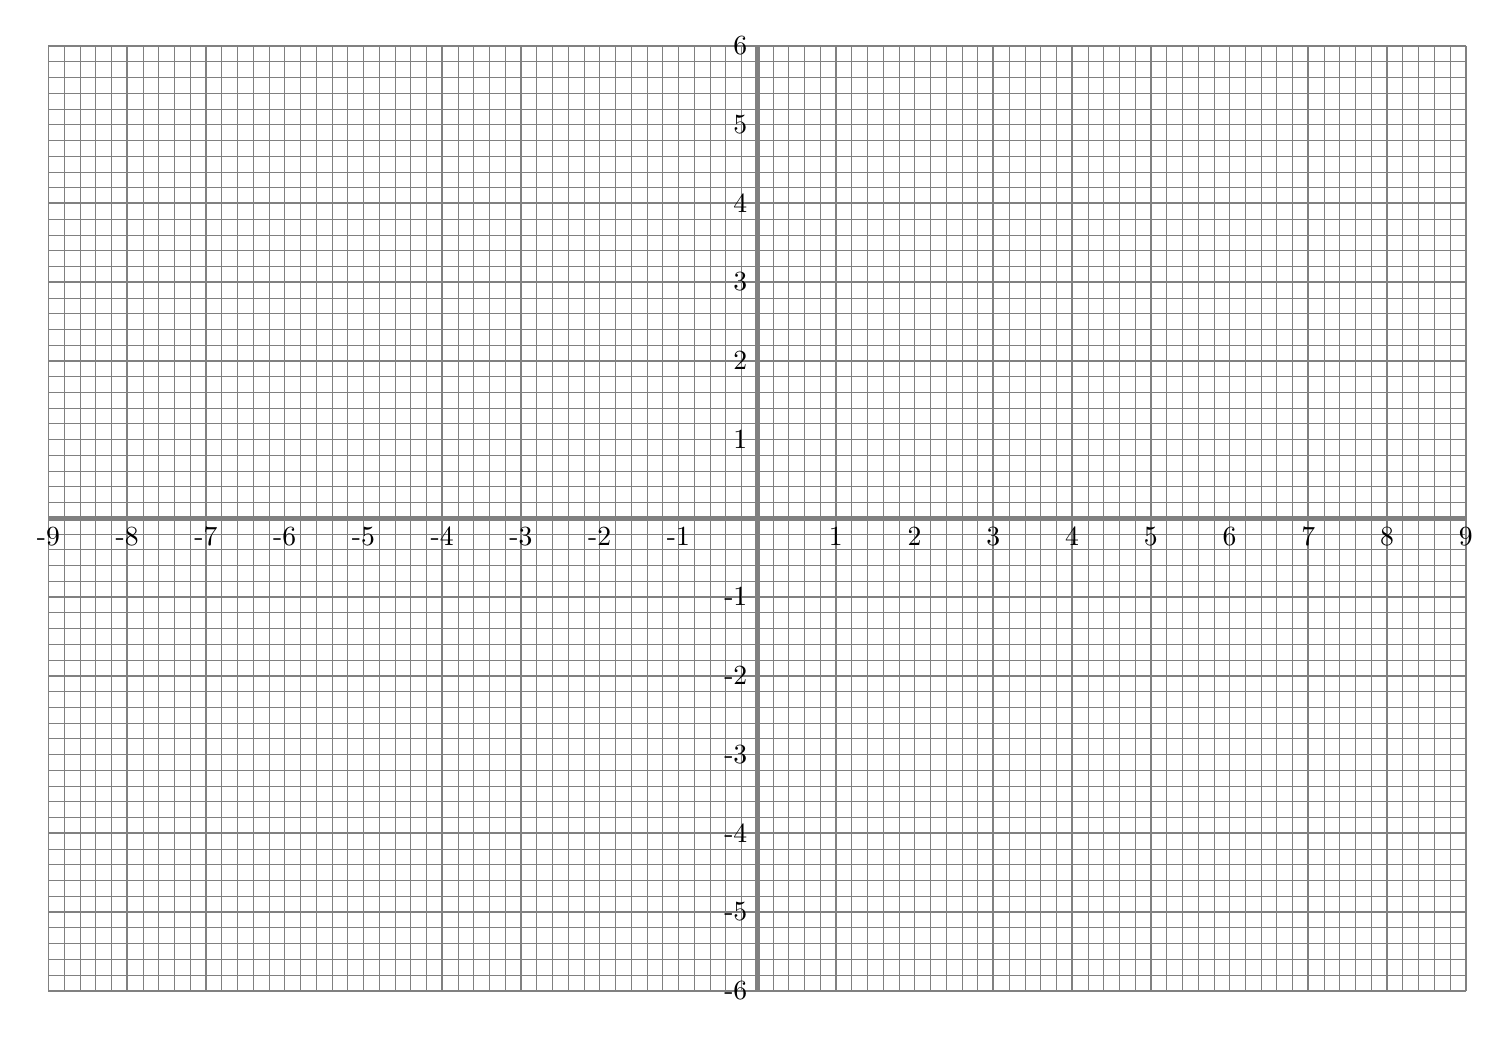
\begin{tikzpicture}
\draw[help lines,step=.2] (-9,-6) grid (9,6);
\draw[help lines,line width=.6pt,step=1] (-9,-6) grid (9,6);
\draw[help lines,line width=1.8pt,step=1] (0,-6) grid (0,6);
\draw[help lines,line width=1.8pt,step=1] (-9,0) grid (9,0);
\foreach \x in {-9,-8,-7,-6,-5,-4,-3,-2,-1, ,1,2,3,4,5,6,7,8,9}
 \node[anchor=north] at (\x,0) {\x};
\foreach \y in {-6,-5,-4,-3,-2,-1, ,1,2,3,4,5,6}
 \node[anchor=east] at (0,\y) {\y};
\end{tikzpicture}

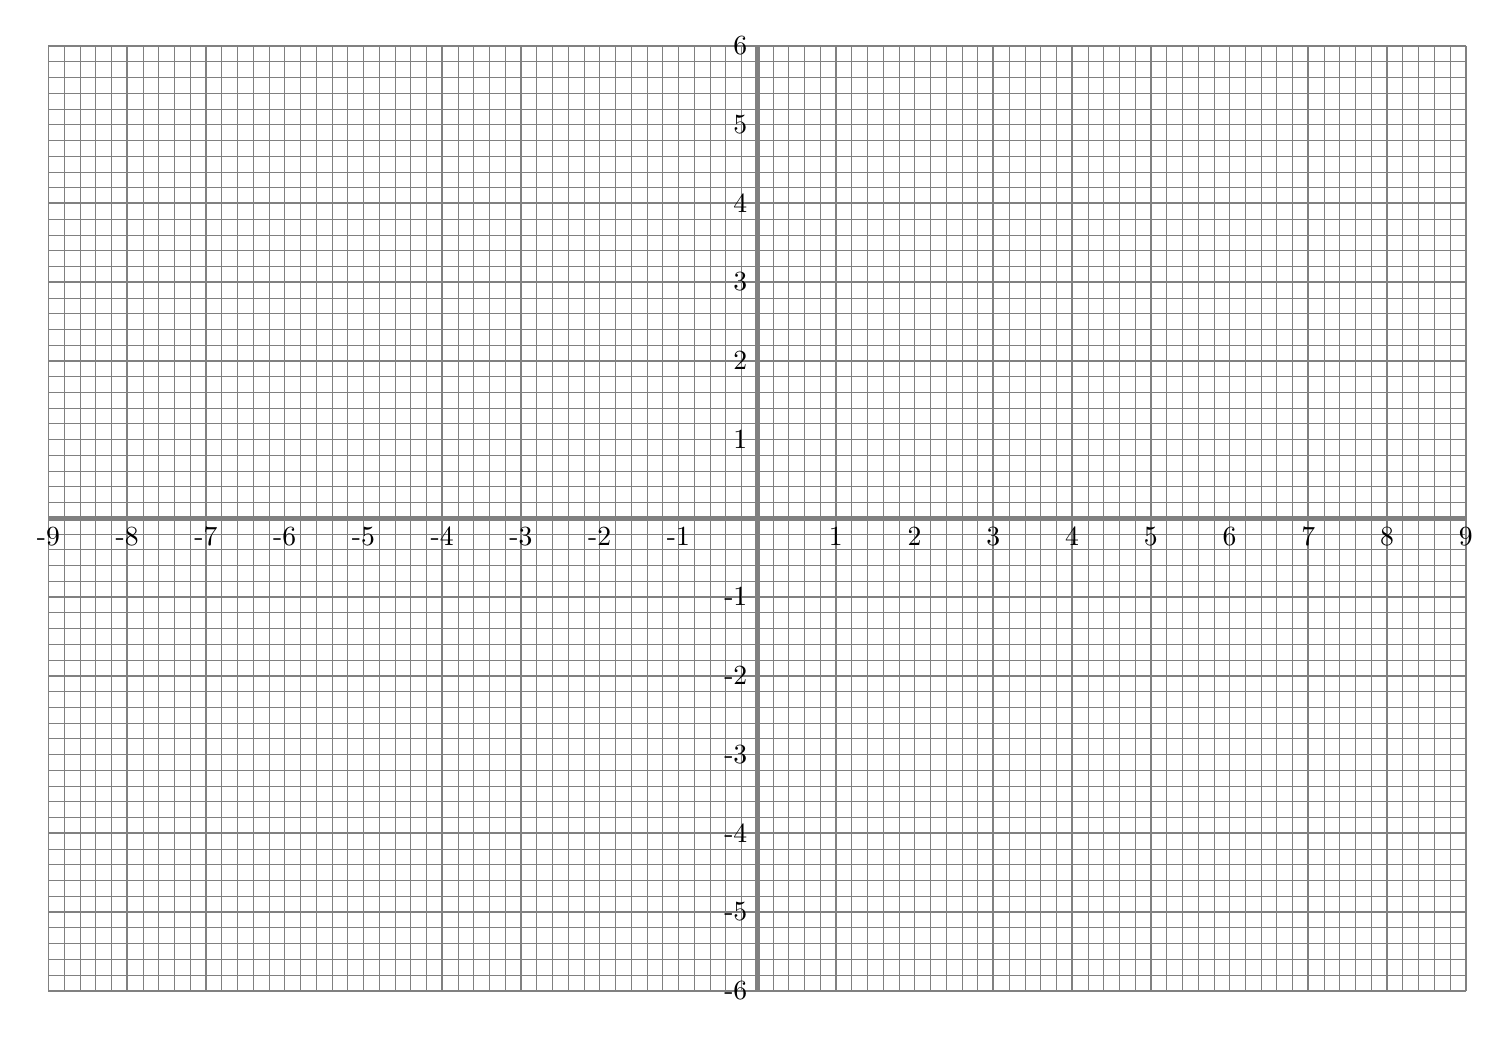
\begin{tikzpicture}
\draw[help lines,step=.2] (-9,-6) grid (9,6);
\draw[help lines,line width=.6pt,step=1] (-9,-6) grid (9,6);
\draw[help lines,line width=1.8pt,step=1] (0,-6) grid (0,6);
\draw[help lines,line width=1.8pt,step=1] (-9,0) grid (9,0);
\foreach \x in {-9,-8,-7,-6,-5,-4,-3,-2,-1, ,1,2,3,4,5,6,7,8,9}
 \node[anchor=north] at (\x,0) {\x};
\foreach \y in {-6,-5,-4,-3,-2,-1, ,1,2,3,4,5,6}
 \node[anchor=east] at (0,\y) {\y};
\end{tikzpicture}

\vphantom
\newline
\newpage
\vphantom
\newline
\newpage
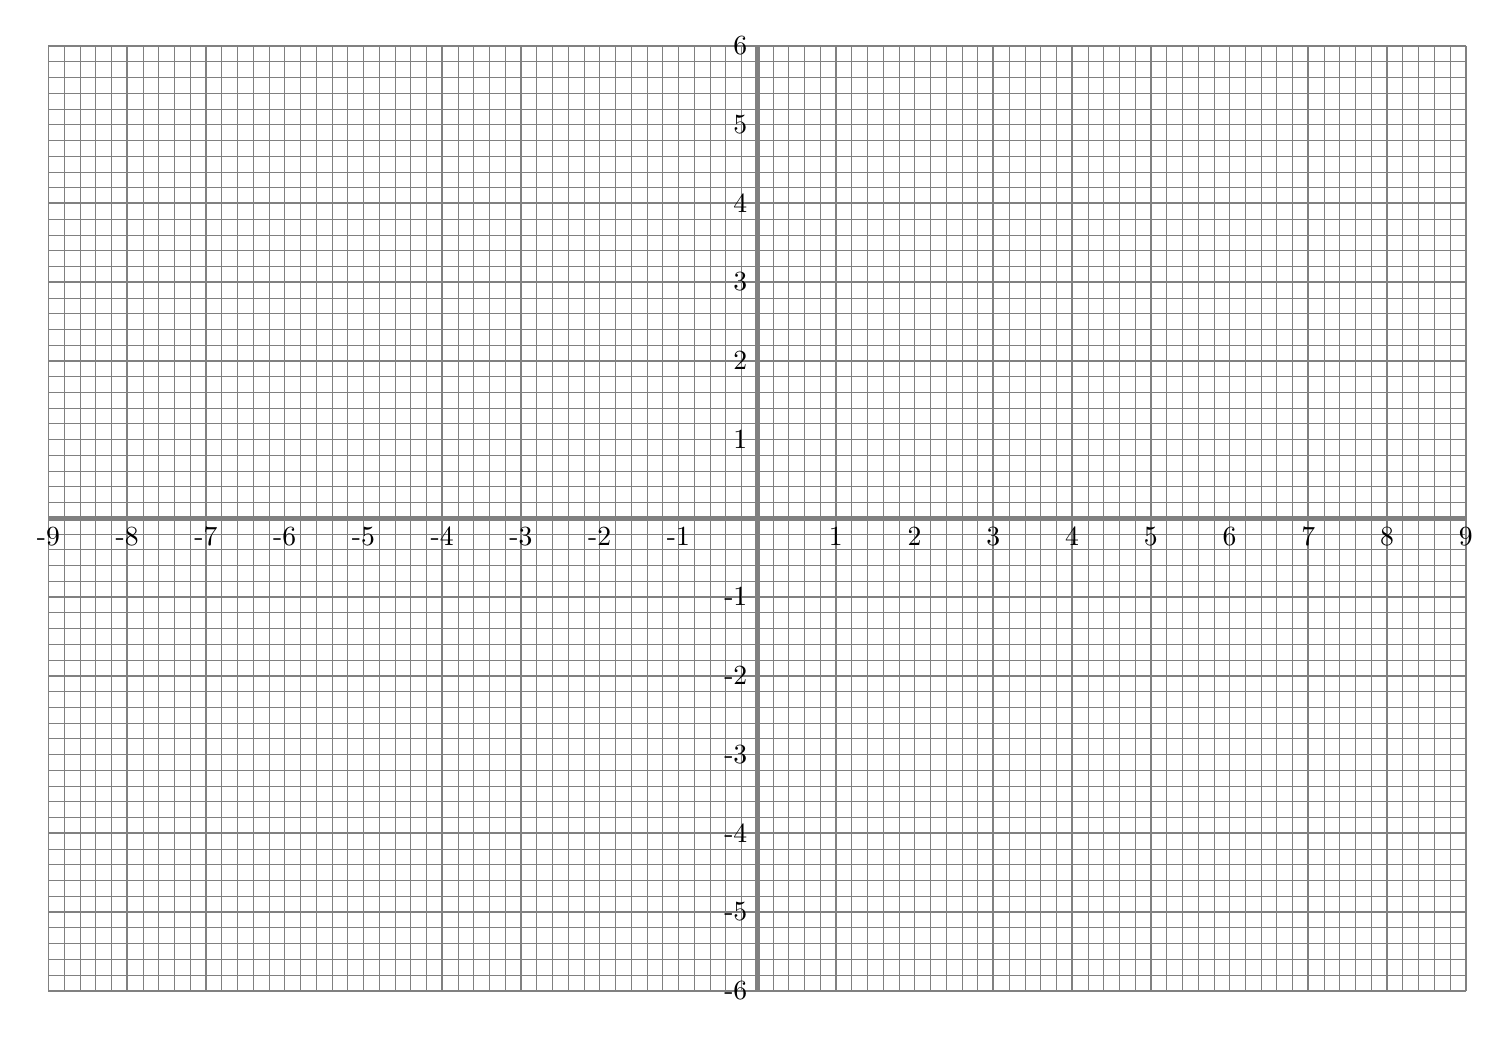
\begin{tikzpicture}
\draw[help lines,step=.2] (-9,-6) grid (9,6);
\draw[help lines,line width=.6pt,step=1] (-9,-6) grid (9,6);
\draw[help lines,line width=1.8pt,step=1] (0,-6) grid (0,6);
\draw[help lines,line width=1.8pt,step=1] (-9,0) grid (9,0);
\foreach \x in {-9,-8,-7,-6,-5,-4,-3,-2,-1, ,1,2,3,4,5,6,7,8,9}
 \node[anchor=north] at (\x,0) {\x};
\foreach \y in {-6,-5,-4,-3,-2,-1, ,1,2,3,4,5,6}
 \node[anchor=east] at (0,\y) {\y};
\end{tikzpicture}

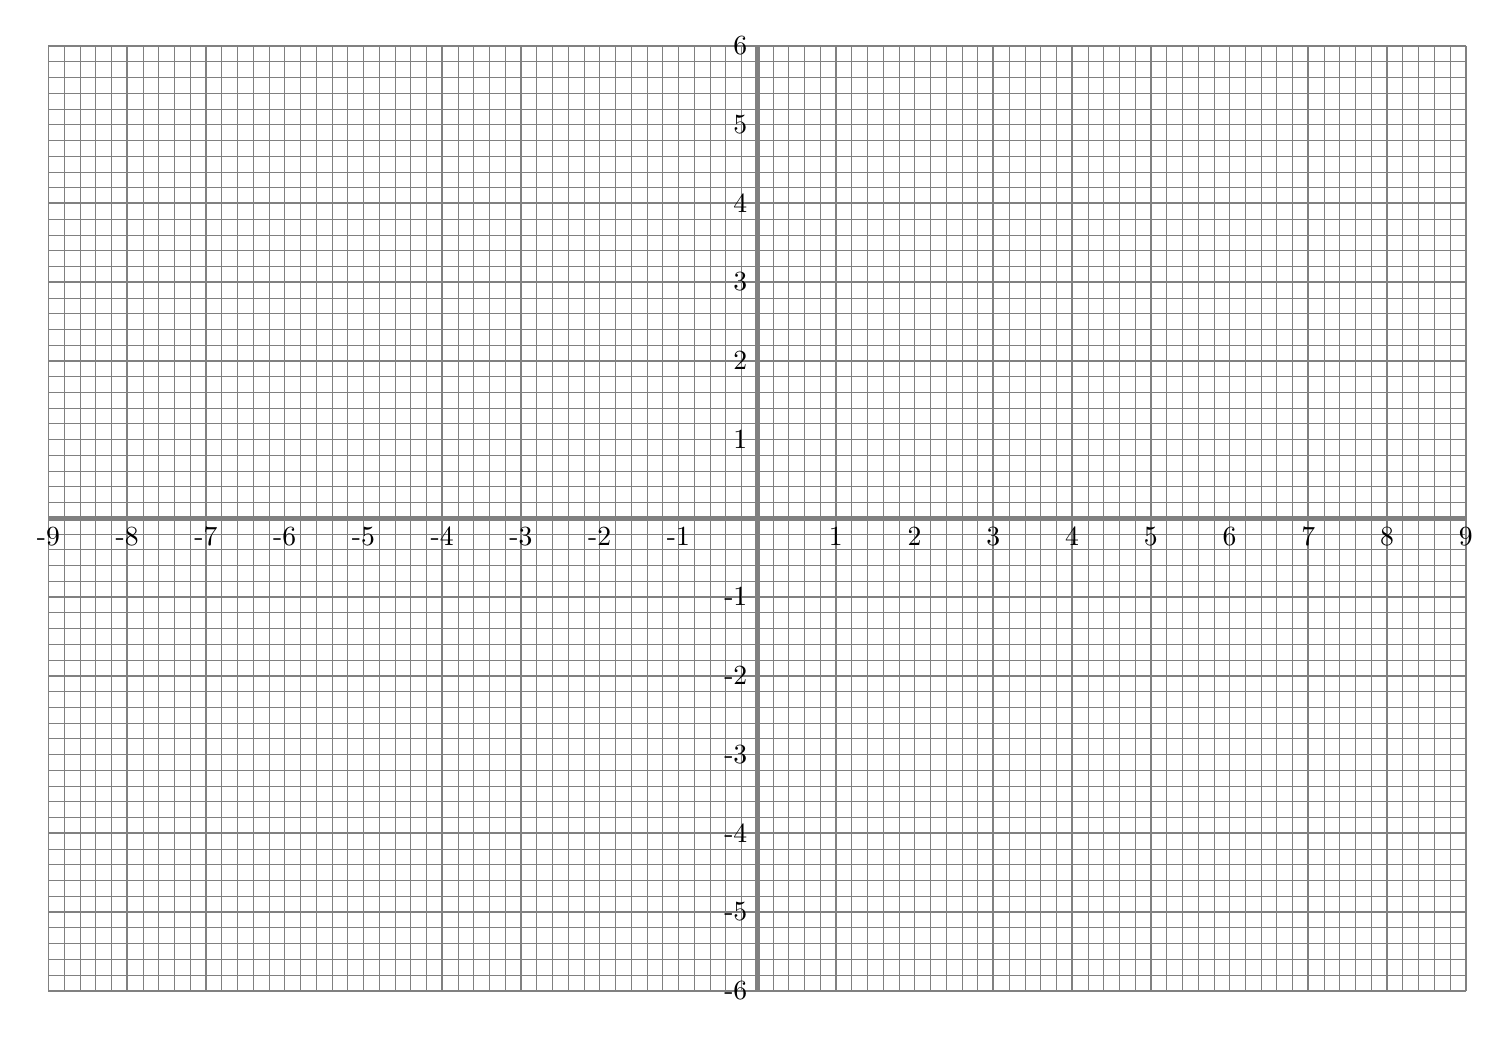
\begin{tikzpicture}
\draw[help lines,step=.2] (-9,-6) grid (9,6);
\draw[help lines,line width=.6pt,step=1] (-9,-6) grid (9,6);
\draw[help lines,line width=1.8pt,step=1] (0,-6) grid (0,6);
\draw[help lines,line width=1.8pt,step=1] (-9,0) grid (9,0);
\foreach \x in {-9,-8,-7,-6,-5,-4,-3,-2,-1, ,1,2,3,4,5,6,7,8,9}
 \node[anchor=north] at (\x,0) {\x};
\foreach \y in {-6,-5,-4,-3,-2,-1, ,1,2,3,4,5,6}
 \node[anchor=east] at (0,\y) {\y};
\end{tikzpicture}

\vphantom
\newline
\newpage
\vphantom
\newline
\newpage
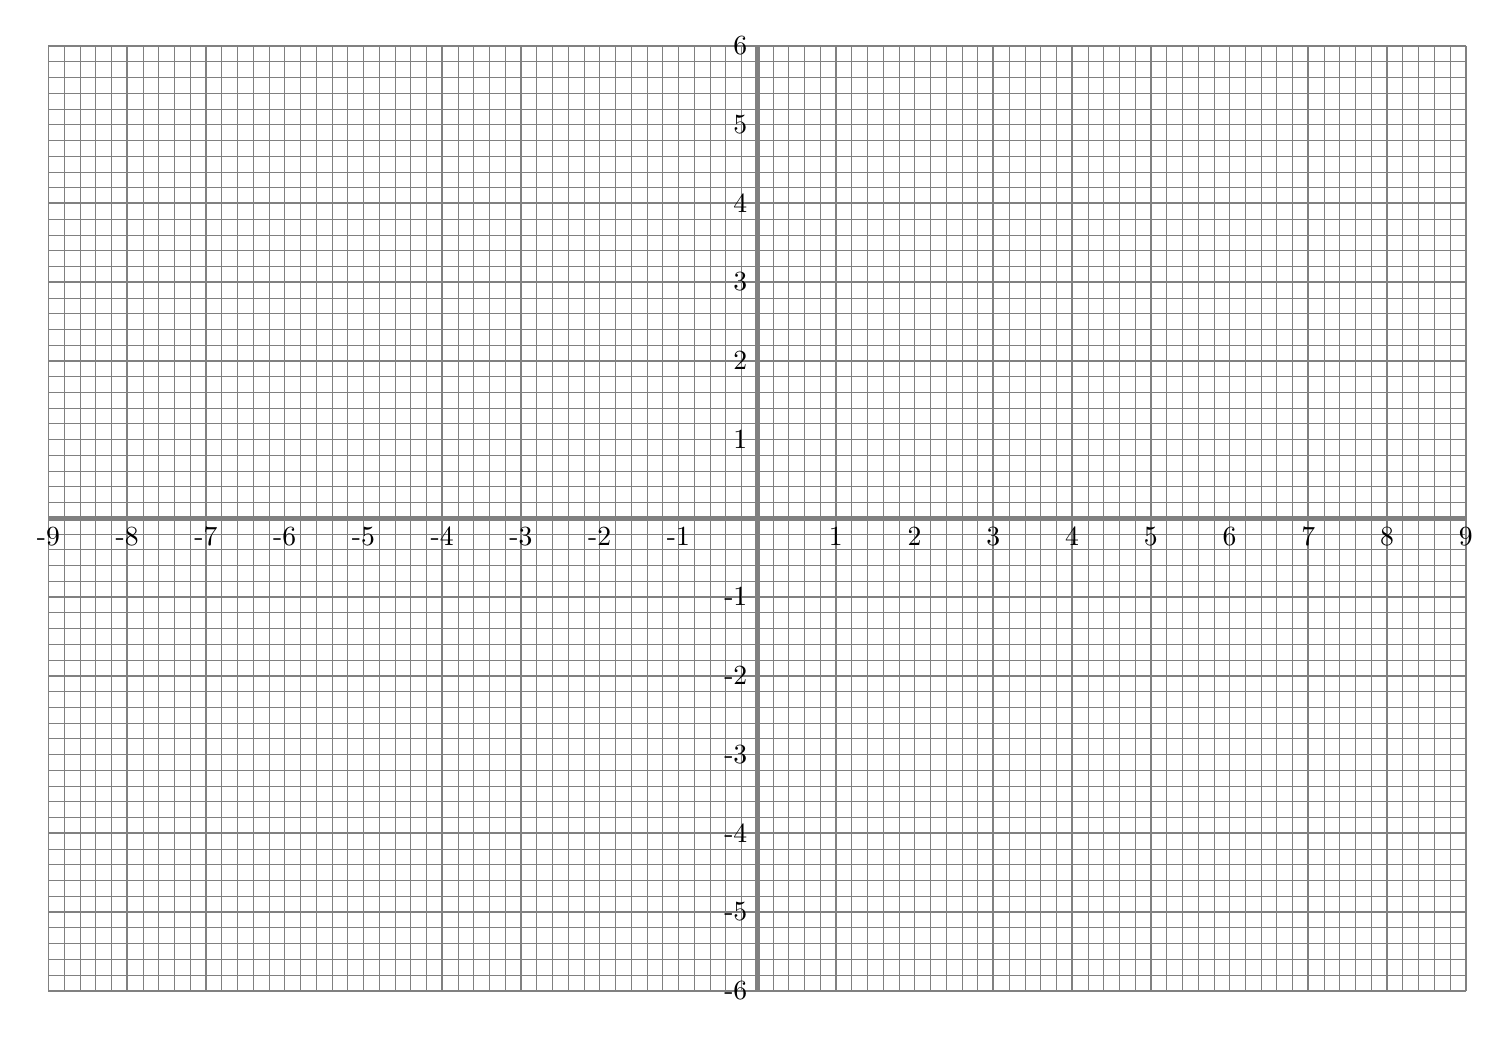
\begin{tikzpicture}
\draw[help lines,step=.2] (-9,-6) grid (9,6);
\draw[help lines,line width=.6pt,step=1] (-9,-6) grid (9,6);
\draw[help lines,line width=1.8pt,step=1] (0,-6) grid (0,6);
\draw[help lines,line width=1.8pt,step=1] (-9,0) grid (9,0);
\foreach \x in {-9,-8,-7,-6,-5,-4,-3,-2,-1, ,1,2,3,4,5,6,7,8,9}
 \node[anchor=north] at (\x,0) {\x};
\foreach \y in {-6,-5,-4,-3,-2,-1, ,1,2,3,4,5,6}
 \node[anchor=east] at (0,\y) {\y};
\end{tikzpicture}

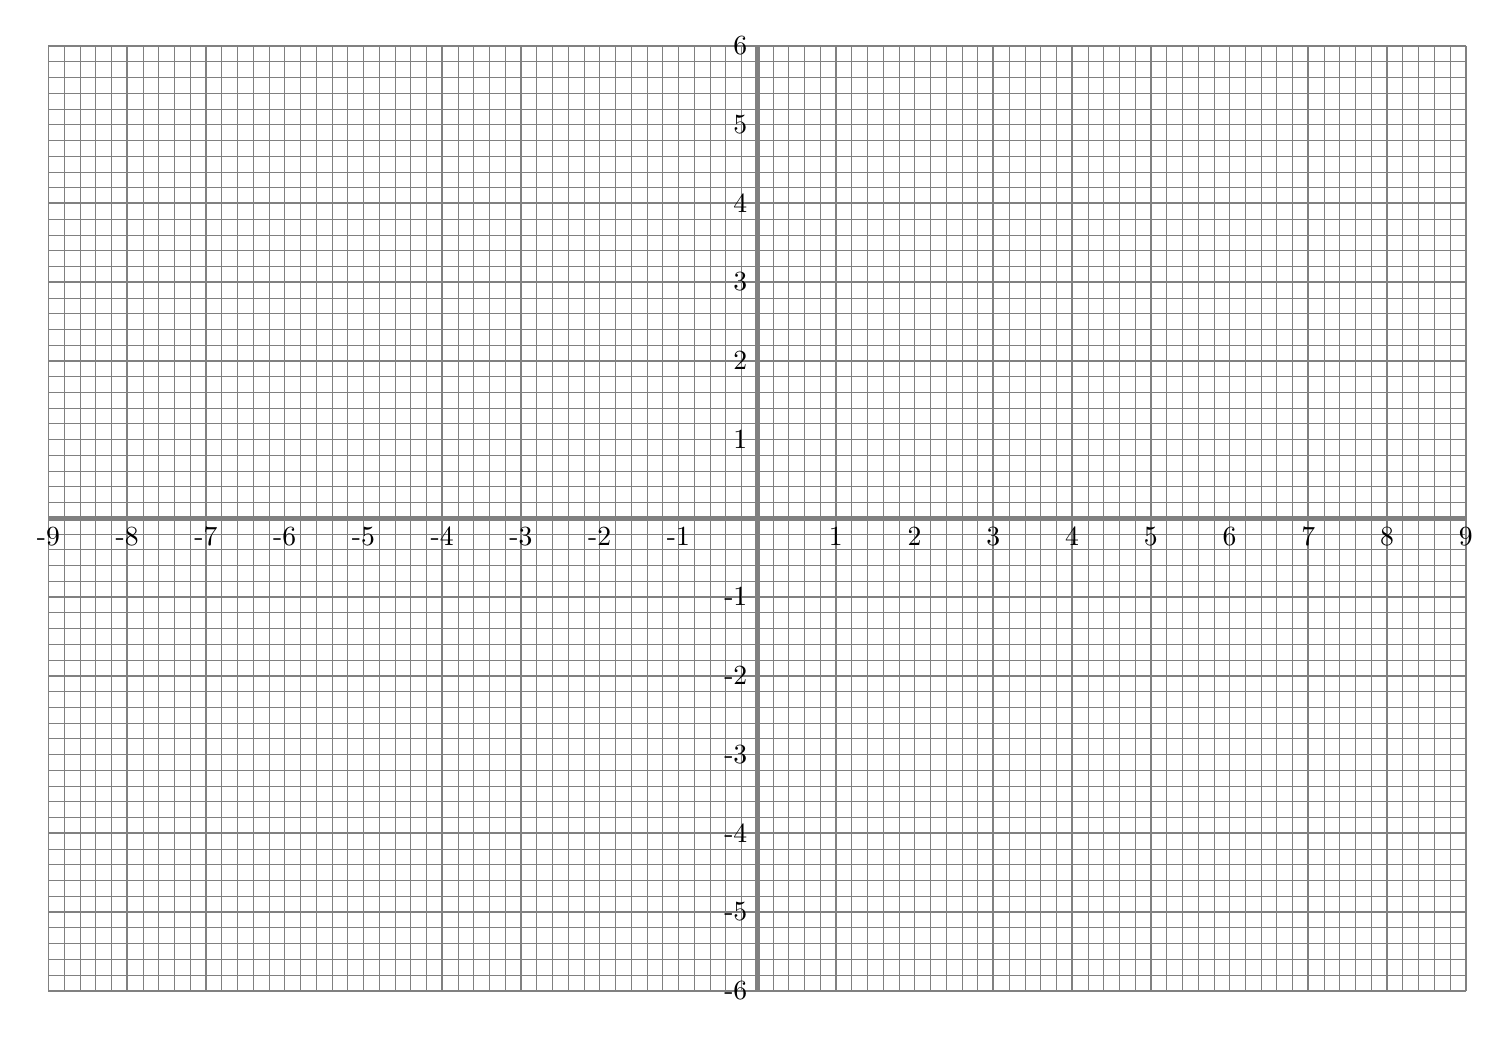
\begin{tikzpicture}
\draw[help lines,step=.2] (-9,-6) grid (9,6);
\draw[help lines,line width=.6pt,step=1] (-9,-6) grid (9,6);
\draw[help lines,line width=1.8pt,step=1] (0,-6) grid (0,6);
\draw[help lines,line width=1.8pt,step=1] (-9,0) grid (9,0);
\foreach \x in {-9,-8,-7,-6,-5,-4,-3,-2,-1, ,1,2,3,4,5,6,7,8,9}
 \node[anchor=north] at (\x,0) {\x};
\foreach \y in {-6,-5,-4,-3,-2,-1, ,1,2,3,4,5,6}
 \node[anchor=east] at (0,\y) {\y};
\end{tikzpicture}

\vphantom
\newline
\newpage
\vphantom
\newline
\newpage
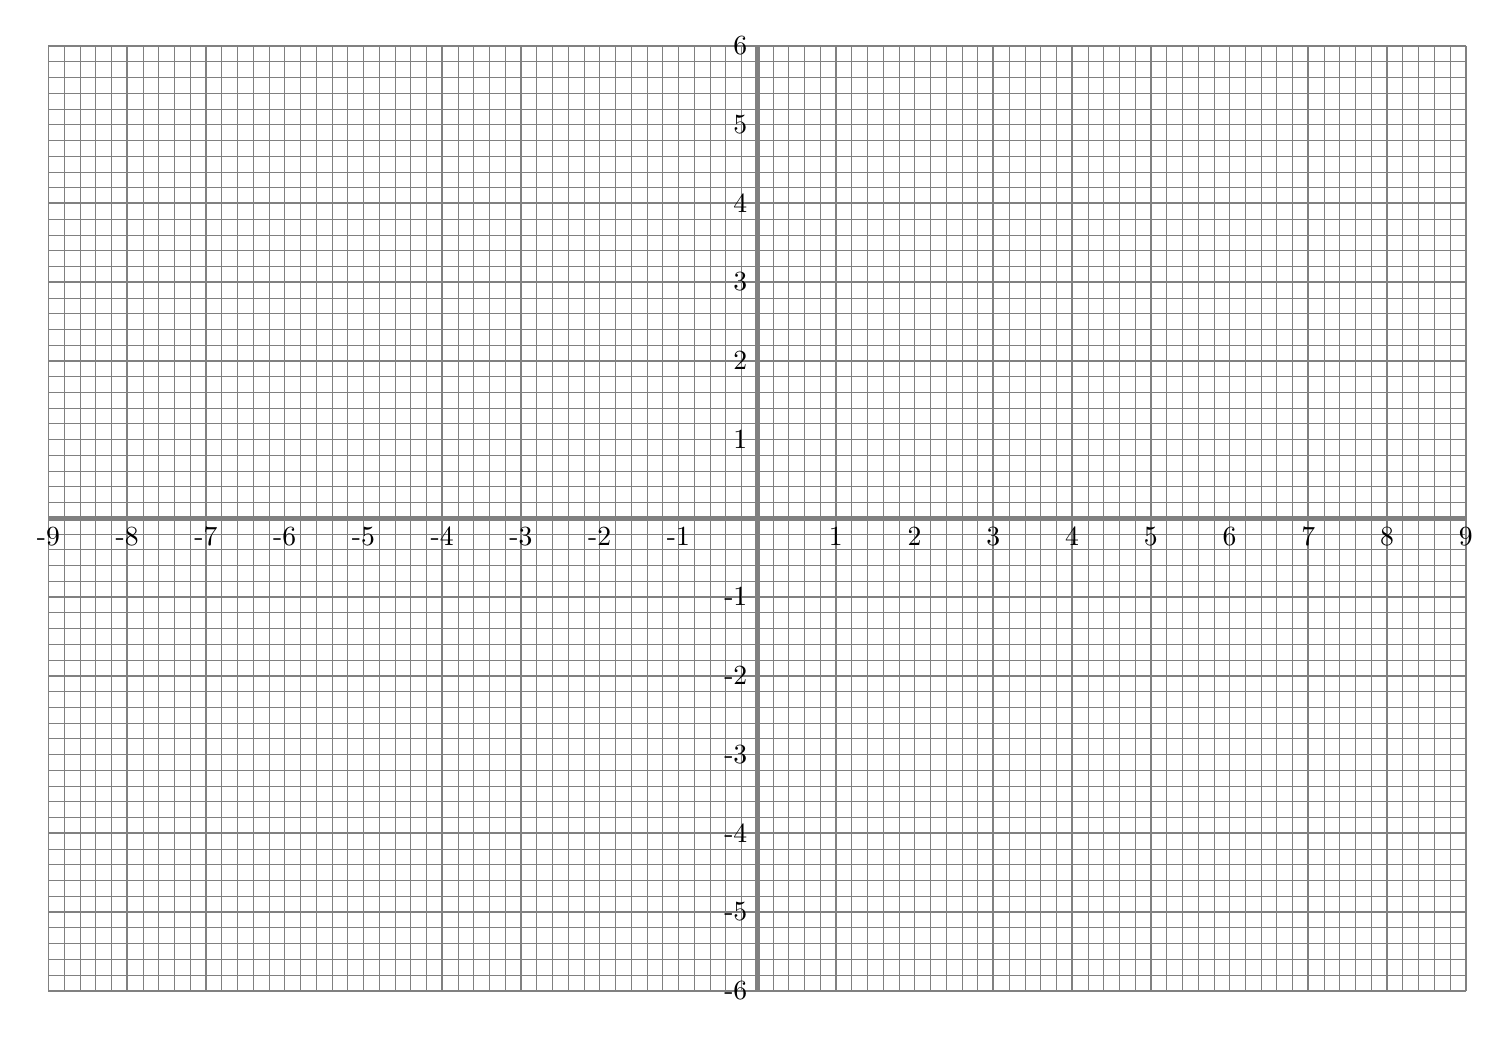
\begin{tikzpicture}
\draw[help lines,step=.2] (-9,-6) grid (9,6);
\draw[help lines,line width=.6pt,step=1] (-9,-6) grid (9,6);
\draw[help lines,line width=1.8pt,step=1] (0,-6) grid (0,6);
\draw[help lines,line width=1.8pt,step=1] (-9,0) grid (9,0);
\foreach \x in {-9,-8,-7,-6,-5,-4,-3,-2,-1, ,1,2,3,4,5,6,7,8,9}
 \node[anchor=north] at (\x,0) {\x};
\foreach \y in {-6,-5,-4,-3,-2,-1, ,1,2,3,4,5,6}
 \node[anchor=east] at (0,\y) {\y};
\end{tikzpicture}

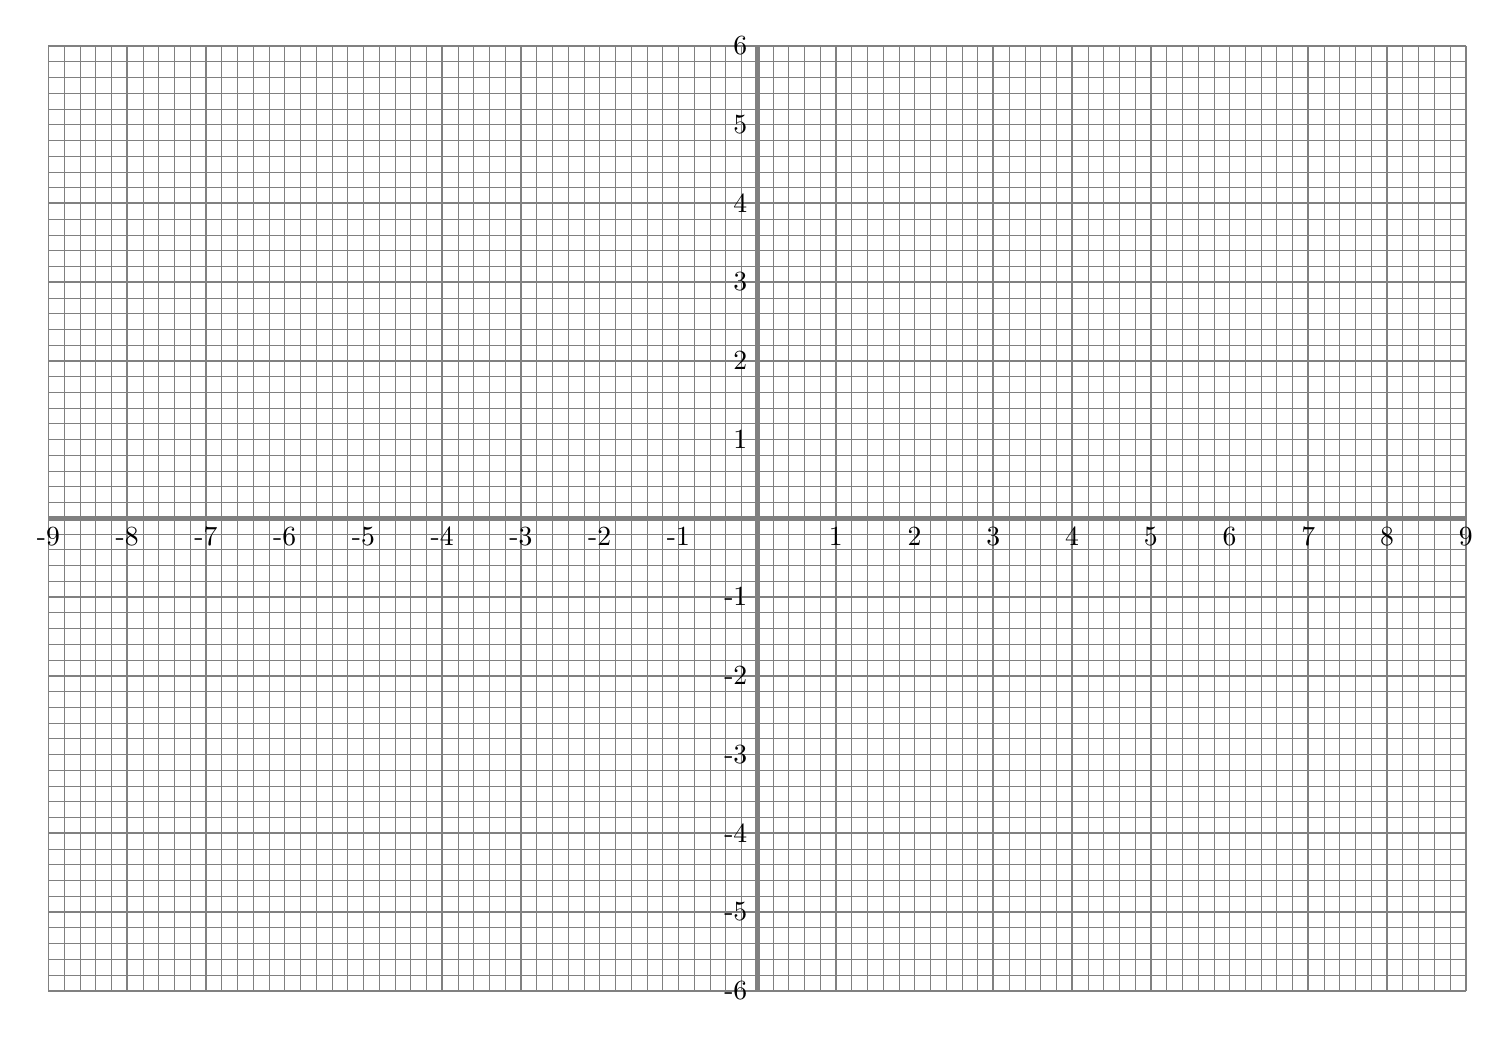
\begin{tikzpicture}
\draw[help lines,step=.2] (-9,-6) grid (9,6);
\draw[help lines,line width=.6pt,step=1] (-9,-6) grid (9,6);
\draw[help lines,line width=1.8pt,step=1] (0,-6) grid (0,6);
\draw[help lines,line width=1.8pt,step=1] (-9,0) grid (9,0);
\foreach \x in {-9,-8,-7,-6,-5,-4,-3,-2,-1, ,1,2,3,4,5,6,7,8,9}
 \node[anchor=north] at (\x,0) {\x};
\foreach \y in {-6,-5,-4,-3,-2,-1, ,1,2,3,4,5,6}
 \node[anchor=east] at (0,\y) {\y};
\end{tikzpicture}

\vphantom
\newline
\newpage
\vphantom
\newline
\newpage
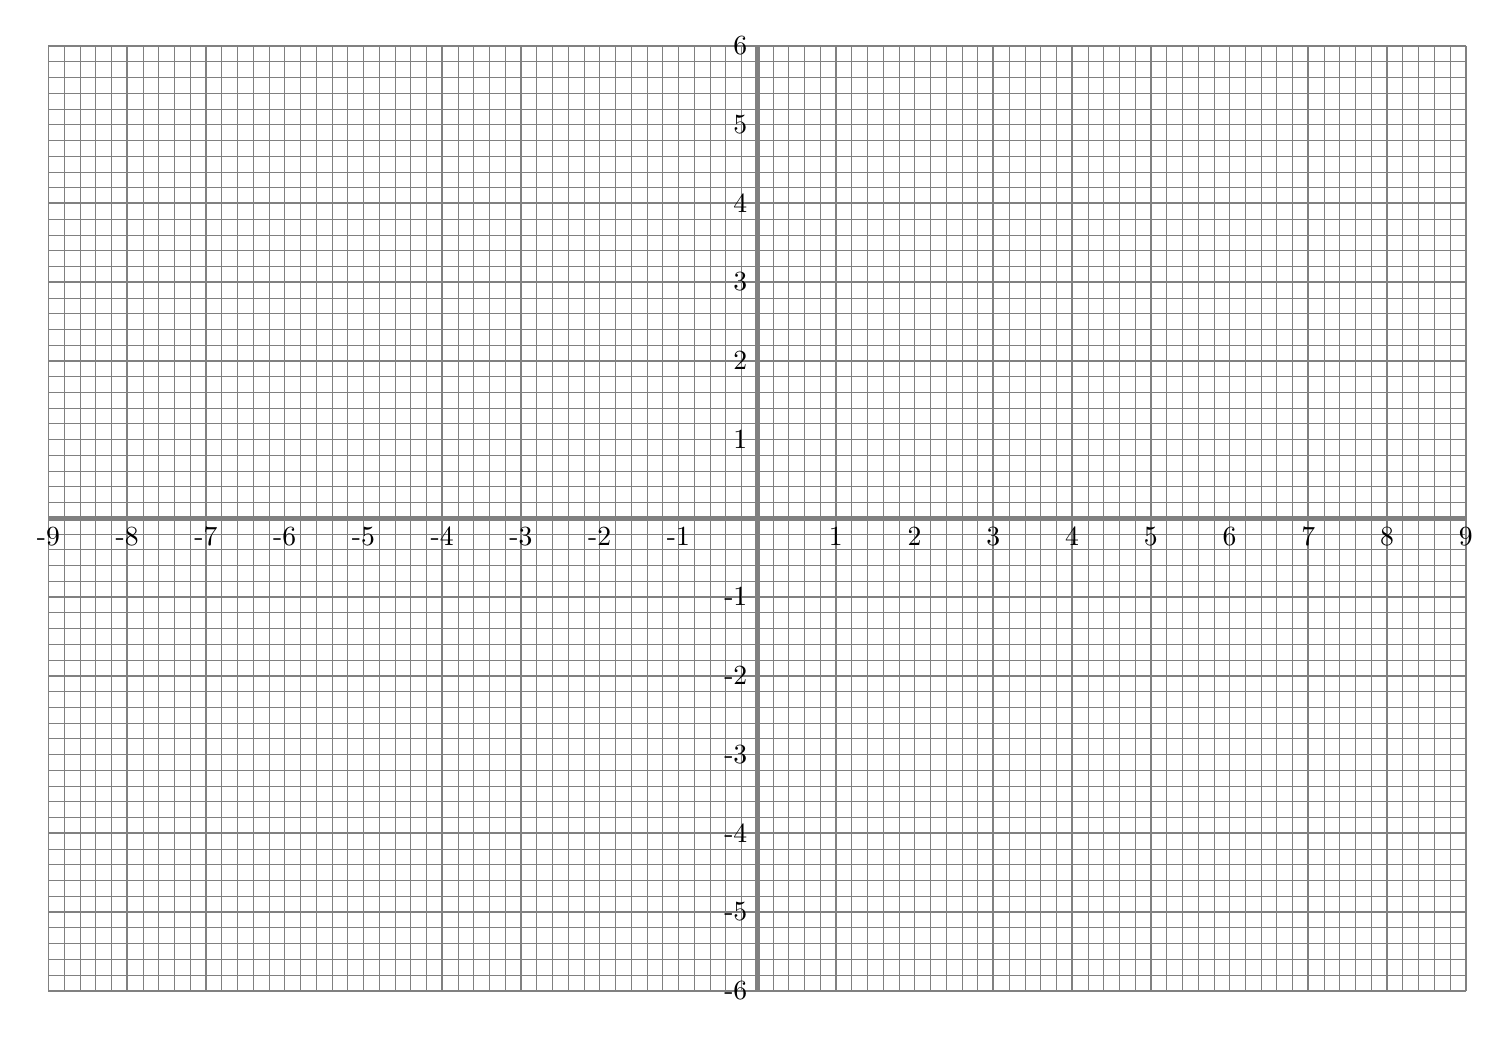
\begin{tikzpicture}
\draw[help lines,step=.2] (-9,-6) grid (9,6);
\draw[help lines,line width=.6pt,step=1] (-9,-6) grid (9,6);
\draw[help lines,line width=1.8pt,step=1] (0,-6) grid (0,6);
\draw[help lines,line width=1.8pt,step=1] (-9,0) grid (9,0);
\foreach \x in {-9,-8,-7,-6,-5,-4,-3,-2,-1, ,1,2,3,4,5,6,7,8,9}
 \node[anchor=north] at (\x,0) {\x};
\foreach \y in {-6,-5,-4,-3,-2,-1, ,1,2,3,4,5,6}
 \node[anchor=east] at (0,\y) {\y};
\end{tikzpicture}

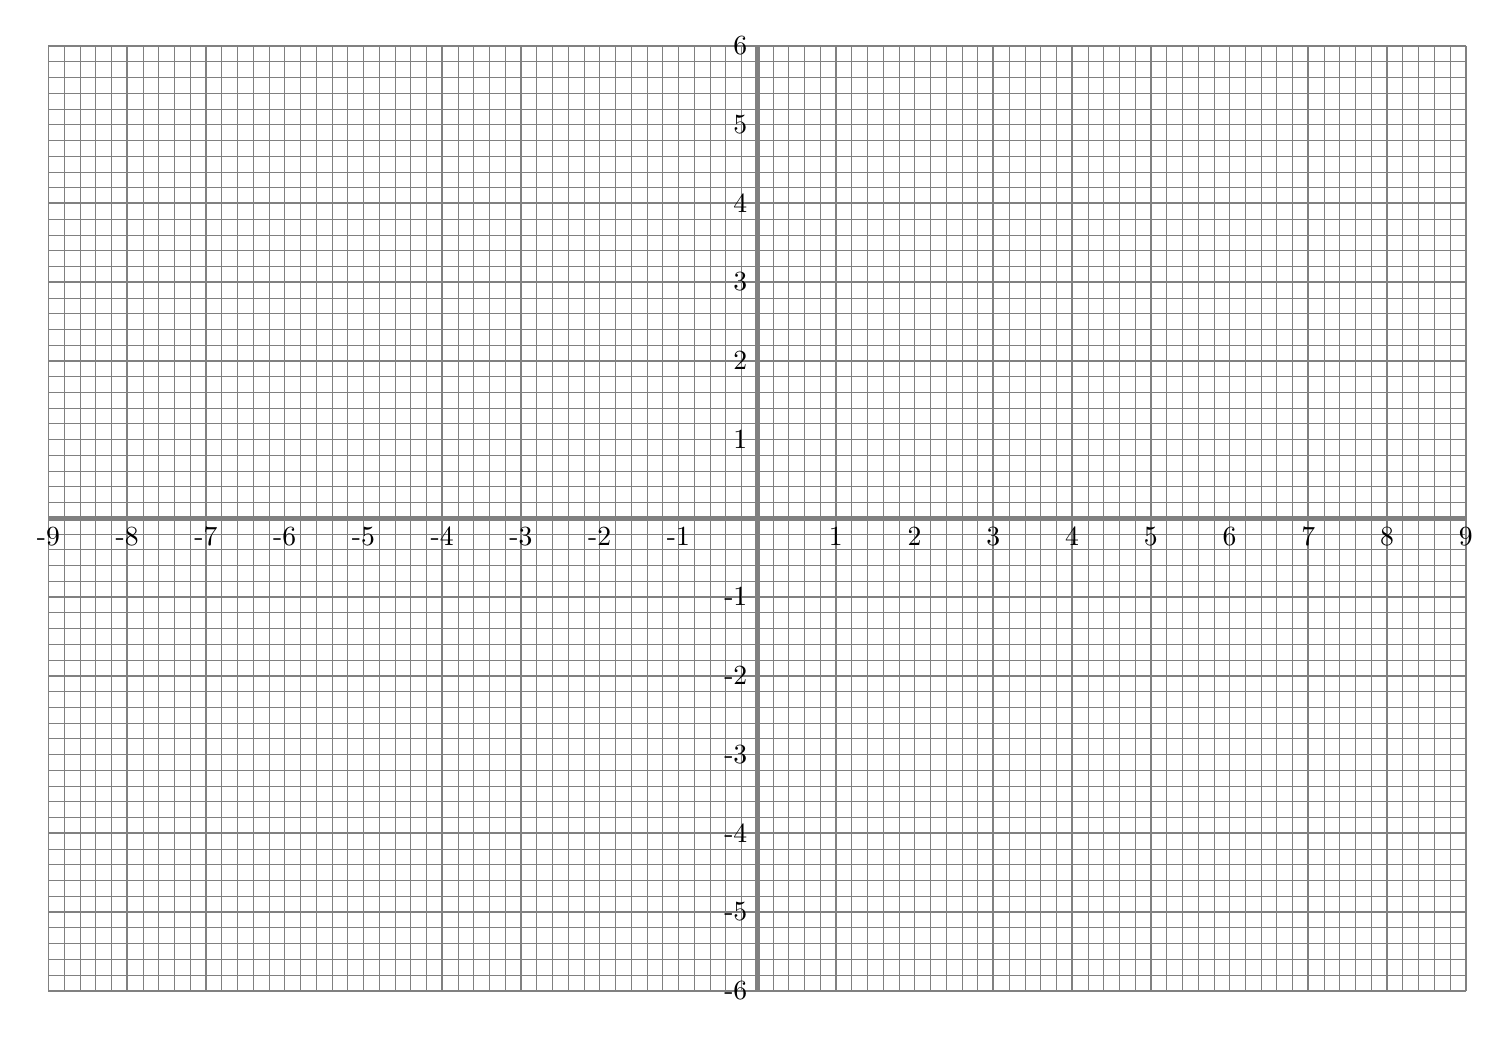
\begin{tikzpicture}
\draw[help lines,step=.2] (-9,-6) grid (9,6);
\draw[help lines,line width=.6pt,step=1] (-9,-6) grid (9,6);
\draw[help lines,line width=1.8pt,step=1] (0,-6) grid (0,6);
\draw[help lines,line width=1.8pt,step=1] (-9,0) grid (9,0);
\foreach \x in {-9,-8,-7,-6,-5,-4,-3,-2,-1, ,1,2,3,4,5,6,7,8,9}
 \node[anchor=north] at (\x,0) {\x};
\foreach \y in {-6,-5,-4,-3,-2,-1, ,1,2,3,4,5,6}
 \node[anchor=east] at (0,\y) {\y};
\end{tikzpicture}

\end{document}



